\documentclass[a4paper,11pt,english]{report}
% Maths packages
\usepackage{verbatim, amsmath, amsfonts, amssymb, amsthm}

% Allows the use of extra characters
\usepackage{textcomp} 

\usepackage[toc,page]{appendix}

% Formatting for URLs
\usepackage{url} 

\usepackage{natbib}

\usepackage{graphicx}

\usepackage[it]{caption}

\usepackage{fancyhdr}
\pagestyle{fancy}
\lhead{}
\chead{}
\rhead{}
\lfoot{}
\cfoot{\thepage}
\rfoot{}
\renewcommand{\headrulewidth}{0pt}
\renewcommand{\footrulewidth}{0pt}

% PDF referencing
\usepackage[
	hyperindex=true,
	pdftitle={Map the Debate},
	pdfauthor={Joseph Root},
	colorlinks=false,
	pagebackref=false,
	citecolor=blue,
	plainpages=false,
	pdfpagelabels
]{hyperref} % colourlinks=false for printing

% Acknowledgements section
% \usepackage{additional/acknowledgements}

% Chapter title's font and spacing
% \usepackage[times]{quotchap}
% \renewcommand*\sectfont{\minionfont\scshape}
% \renewcommand{\chapterheadstartvskip}{\vspace*{-2.5\baselineskip}}
% \renewcommand*{\chapterheadendvskip}{\vspace{1.3\baselineskip}}

% Packages for type setting
\usepackage{fontspec}
\usepackage[parfill]{parskip}
\usepackage{titlesec}
\usepackage{titling}
\usepackage{textcase}
\usepackage{color}
\usepackage[british]{babel}
\usepackage{setspace}

% Basic typesetting
\setmainfont[Mapping=text-text, Ligatures={Common}]{Adobe Caslon Pro}
\setromanfont[Mapping=text-text, Ligatures={Common}]{Adobe Caslon Pro}
\setmonofont[Scale=0.78]{Menlo}
\setlength{\parindent}{9pt}

% Initialise font families
\newfontfamily\minionfont[Mapping=text-text, Ligatures={Common}]{Minion Pro}
\newfontfamily\trajanfont[Mapping=text-text, Ligatures={Common}]{Trajan Pro}
\newfontfamily\sabonfont[Mapping=text-text, Ligatures={Common}]{Sabon LT Std}
\newfontfamily\caslonfont[Mapping=text-text, Ligatures={Common}]{Adobe Caslon Pro}
\newfontfamily\minionoldfont[Mapping=text-text, Ligatures={Common}, Numbers=OldStyle]{Minion Pro}
\newfontfamily\dinfont[Mapping=text-text, Ligatures={Common}]{DIN 30640 Std}
\newfontfamily\museofont[Mapping=text-text, Ligatures={Common}, Scale=1.2]{Museo Sans 100}
\newfontfamily\consolasfont[Scale=0.78]{Menlo}

% Section title's font and style
\titleformat*{\section}{\Large\minionoldfont\addfontfeature{LetterSpace=2}}
\titleformat*{\subsection}{\large\minionoldfont\addfontfeature{LetterSpace=2,Scale=1.1}}
\titleformat*{\subsubsection}{\normalsize\itshape\minionoldfont\addfontfeature{Scale=1.05}}

\titlespacing*{\chapter}{0pt}{-30pt}{30pt}
\titleformat{\chapter}[display]
	{\flushright\Huge\color{grey}\sabonfont\addfontfeature{Scale=4.5}\bfseries}
	{\thechapter}
	{10pt}
	{\normalfont\flushright\LARGE\color{black}\minionfont\scshape\MakeUppercase}

\titleformat{\part}[display]
  {\LARGE\color{darkgrey}\minionfont\addfontfeature{LetterSpace=3}\scshape}
  { }
  {3em}
	{\MakeUppercase\partname{} \thepart\MakeUppercase { } \vline { }  \color{black}\MakeUppercase}


\definecolor{lightblue}{RGB}{144,164,174}
\definecolor{darkgreen}{RGB}{72,146,0}
\definecolor{lightred}{RGB}{169,53,53}
\definecolor{grey}{gray}{0.55}
\definecolor{darkgrey}{gray}{0.45}

% Code formatting
\usepackage{listings}
\lstloadlanguages{Ruby}
\lstset{
	basicstyle=\consolasfont\color{black},
	numbers=left,
	numberstyle=\consolasfont\addfontfeature{Scale=0.73}\color{darkgrey},
	commentstyle=\color{darkgreen},
	keywordstyle=\color{blue},
	stringstyle=\color{lightred},
	frame=lines,
	framesep=6pt,
	abovecaptionskip=6pt,
	belowcaptionskip=6pt,
	breaklines=true,
	tabsize=2,
	showspaces=false,
	showstringspaces=false,
	captionpos=t
}

\usepackage[titles]{tocloft}
\setlength{\cftbeforechapskip}{1ex}
\setlength{\cftbeforesecskip}{0.5ex}

\usepackage{longtable}
\usepackage{array}
\usepackage{multirow}

\usepackage{float}
\floatplacement{figure}{H}

\setcounter{secnumdepth}{3}

\DeclareMathOperator*{\argmax}{arg\,max}
\DeclareMathOperator*{\occurences}{occurences}
\DeclareMathOperator*{\pos}{pos}

% Details for cover page
\author{Joseph Root\\
Imperial College, London\\
jsr08@ic.ac.uk}
\date{June 2011}
\title{Map the Debate}

% \includeonly{title/title, background/background, introduction/introduction, overview/overview}

\begin{document}
	
	\begin{titlepage}

\begin{center}

\vspace*{\fill}
% Upper part of the page


\minionfont\addfontfeature{Scale=1.1}\Huge Map the Debate \\[0.3cm]

\caslonfont\addfontfeature{Scale=1.1}\normalsize Understanding the web's response \\[1cm]

\caslonfont

\emph{Author:} Joseph Root <jsr08@ic.ac.uk>\\
\emph{Supervisor:} Francesca Toni <f.toni@ic.ac.uk>\\ [1cm]
June 2011 \\[3cm]


% 
% % Title
%  \\[0.4cm]
% { \huge \bfseries Lager brewing techniques}\\[0.4cm]
% 
% \\[1.5cm]
% % Author and supervisor
% \begin{minipage}{0.4\textwidth}
% \begin{flushleft} \large
% \emph{Author:}\\
% John \textsc{Smith}
% \end{flushleft}
% \end{minipage}
% \begin{minipage}{0.4\textwidth}
% \begin{flushright} \large
% \emph{Supervisor:} \\
% Dr.~Mark \textsc{Brown}
% \end{flushright}
% \end{minipage}

\vspace*{\fill}

% Bottom of the page
\scshape Imperial College London

\end{center}

\end{titlepage}
	
	\chapter*{acknowledgements}

I would like to thank my parents, girlfriend Elizabth, Tim (sorry!) and Catherine for all their support over the past few months. I can't tell you how much of a difference each one of you has made. I'd like to thank Susan Eisenbach for her continual advice, support and open door over the past three years. Thanks also to my second marker, Iian Phillips, for his willingness to help and general input to the project. 
	
Lastly, I would like to thank my supervisor Francesca Toni. Your insightful input, enthusiasm and encouragement have kept me going on the numerous occasions I've felt like giving up. Thank you for taking on my project, its (sp?) genuinely been a pleasure!
	
	\begin{abstract}
	Some abstract
	
\end{abstract}
	
	\setcounter{tocdepth}{1}
	\tableofcontents
	
	\part{Analysis}
	
	% This is one of the most important components of the report. It should begin with a clear statement of what the project is about so that the nature and scope of the project can be understood by a lay reader. It should summarise everything you set out to achieve, provide a clear summary of the project's background, relevance and main contributions. It should explain the motivation for the project (i.e., why the problem is important) and identify the issues to be addressed (i.e., why the problem is difficult). The introduction should set the scene for the project and should provide the reader with a summary of the key things to look out for in the remainder of the report. When detailing the contributions it is helpful to provide pointers to the section(s) of the report that provide the relevant technical details. The introduction itself should be largely non-technical. It is sometimes useful to state the main objectives of the project as part of the introduction. However, avoid the temptation to list low-level objectives one after another in the introduction and then later, in the evaluation section (see below), say something like "All the objectives of the project have been met blah blah...". A project that meets all its objectives is, by definition, weak and unambitious. Concentrate instead on the big issues, e.g. the main questions (scientific or otherwise) that the project sets out to answer.

\chapter{Introduction}

% The ability to listen to and understand public opinion serves as the foundation upon which democratic society is built. Although the merits of different electoral systems can be debated, in general they all provide effective and functional methods for democratically electing governments. 

\section{Motivation}

From women's rights to civil rights, the influence of public opinion on government policy has been pivotal. Within a healthy democracy the voice of the electorate should be heard and recognised by those chosen to represent them. Throughout history platforms have often been provided for public opinion to be made known, from the early public forums of Greece and Rome, to speaker's corner and the house of commons today. Providing a means for people to express their opinion enables them to both challenge and shape the direction their elected governments take. As a result, finding ways of gathering and understanding this opinion has increasingly proven fundamental if a government wishes to be successful.

Current methods of measuring opinion are largely statistical, with methods such as polling looking at the opinion of a sample group, before using their results to make further predictions. These can be informative, however their small sampling rates mean that figures can often be askew. Furthermore polling is both costly and time consuming to conduct, and thus can neither be used to find opinion on breaking news or across a large number of topics. None the less, as methods for measuring public opinion have improved both in accuracy and detail, politicians and policy makers have increasingly turned to them not only for affirmation of their policies, but for guidance and new initiative.

As the web has become more prevalent throughout society, it is increasingly becoming a platform for discussion and opinion. The initial growth of blogging demonstrated the web's ability to serve as a forum for debate and opinion. However the technical knowledge required to start a blog, alongside the time required to write a post meant that adoption was limited. In the past two years we have seen the rise of micro-blogging (essentially 140 character blog posts) through services such as Twitter. These have seen unprecedented levels of adoption, with Twitter's 200 million users posting 25 billion micro-blog posts in 2010. Due to the simple nature of writing short posts, micro-blog discussion tends to break quickly around news topics, and offers genuine insight into public opinion surrounding news topics.

This project hopes to utilise the growth of publicly available opinion on the web, using it as a source upon which new methods for analysing and measuring public opinion can be built. In particular the project will focus on understanding sentiment on micro-blogging services such as Twitter. 

\section{Contributions}

\begin{enumerate}

\item Ruby implementation of a sentiment analysis engine based upon current research. The engine should be able to correctly identify sentences containing sentiment, and classify the sentiment as positive or negative. Different implementations should be tested and compared to determine which algorithms and techniques work best.

\item An algorithm for classifying sentiment as a range of emotion and feeling, rather than just a score along a scale of positive to negative. The algorithm should be implemented in Ruby and included in the sentiment analysis engine.

\item Research optimisations for current algorithms, in order to tailor the sentiment analysis engine for micro-blog posts from services such as Twitter. These optimisation should be implemented within the engine.

\item Research optimisations for current algorithms, in order to better facilitate the understanding of Politically focussed micro-blog data. These optimisation should be implemented within the engine.

\item A Ruby based Twitter module to store and classify live data from Twitter. 

\item Visualisations should be designed and implemented to help better understand the data and classification results.

\end{enumerate}
	
	% The background section of the report should set the project into context by relating it to existing published work which you read at the start of the project when your approach and methods were being considered. There are usually many ways of solving a given problem, and you shouldn't just pick one at random. Describe and evaluate as many alternative approaches as possible. The published work may be in the form of research papers, articles, text books, technical manuals, or even existing software or hardware of which you have had hands-on experience. Your must acknowledge the sources of your inspiration. You are expected to have seen and thought about other people's ideas; your contribution will be putting them into practice in some other context. However, avoid plagiarism: if you take another person's work as your own and do not cite your sources of information/inspiration you are being dishonest; in other words you are cheating. When referring to other pieces of work, cite the sources where they are referred to or used, rather than just listing them at the end. Make sure you read and digest the Department's plagiarism document .

% In writing the Background chapter you must demonstrate your capability of analysis, synthesis and critical judgement. Analysis is shown by explaining how the proposed solution operates in your own words as well as its benefits and consequences. Synthesis is shown through the organisation of your Related Work section and through identifying and generalising common aspects across different solutions. Critical judgement is shown by discussing the limitations of the solutions proposed both in terms of their disadvantages and limits of applicability.

\chapter{Background}
\label{background}

From it's early forums through to the 'social web' of today, the Internet has served as a continually expanding platform for discussion. The result has been an explosion in the amount of readily available, computer-formatted textual opinion. With this growth has come an increasing desire to computationally understand the wealth of opinion now so easily accessible. Combining elements of linguistics, natural language processing and machine learning, this field of exploration has come to be known as \emph{opinion mining} or \emph{sentiment analysis}. In the following chapter we will first briefly examine Twitter as a backdrop to our discussion on sentiment analysis. We will then go on to explore the general problems posed by sentiment analysis along with the common approaches and solutions taken in addressing them. In sections \ref{background:discovering_opinion} - \ref{background:topic_extraction} we will discuss in detail the areas and methods of sentiment analysis which will bear relevance to this project's Twitter-based setting. Finally in section \ref{background:emotion} we will explore emotion in general, particularly looking at it's scope and ways of classifying it.

\section{Twitter}
\label{background:twitter}

Twitter is a social-networking web-service. It enables users to post and read 140 character messages known as \emph{tweets}. A user's \emph{timeline} serves as a publicly viewable history of their tweets. Furthermore if someone chooses to \emph{follow} another user, they will be notified of changes to that user's timeline. This simplicity has seen Twitter's user-base rapidly expand, with over 200 million active users today. From football transfers to revolutions Twitter has become the go-to service for spreading news quickly and efficiently.

Since its launch in 2006, certain protocols have emerged from within the Twitter community. These have been embraced by Twitter, enabling it to serve not only as an efficient platform for spreading news, but also as a rich and sophisticated medium for conversation. Notable protocols include:

\begin{description}
	\item [Hashtags] enable users to tag their tweets with any word or combination of characters they deem appropriate. Although this may seem basic at first, through common hashtags, it enables users to take part in a community-wide discussion. For example, during the recent voting reform referendum, the hashtags '\emph{\#yes2av}' and '\emph{\#no2av}' were used to form a debate on the strengths and weaknesses of the Alternative Vote. 
	\item [Mentions] allow users to reference other users in their tweets. Furthermore if a user is mentioned in a tweet, Twitter will notify the mentioned user. Through this, Twitter users can take part in a direct conversations with one or more other users. For example, if we wanted to ask Stephen Fry a question, we could tweet '\emph{what are you eating for breakfast @stephenfry?}'.
	\item [Re-tweets] give users the ability to re-post other users' tweets in their own timeline. This simple feature has had a significant impact on Twitter's ability to facilitate the rapid spread of news. For example in 2009 when the US Airways flight 1549 crash landed in the Hudson river, rapid re-tweeting of an amateur photo meant the news broke on Twitter far earlier than it did within the media at large. This has continued to be true for many more notable events such as the recent North-African revolutions.
	\item [Links] have always been the popular subject of tweets, however the introduction of link-shorteners has changed the way in which they are posted. In freeing up characters by shortening a URL, users now have the option to describe or comment on the link they are tweeting. This has enabled users to engage in deeper conversation on content they have viewed online, and has neatly allowed Twitter's viral nature to better merge with it's community's desire for debate.
\end{description}

Through Twitter's RESTful API \footnote{RESTful API's allow developers to retrieve, modify, create and delete data by making get, post and delete HTTP requests to specified web addresses.}, this rich resource of live news and debate will serve as the project's main data source.

\section{Sentiment analysis}
\label{background:sentiment_analysis}

Sentiment analysis as a field, is the exploration of how we can computationally understand opinions expressed within a body of text. In order to do this, we must first define a computational structure for expressing opinions. In general \cite{Liu:2010tm} this is done by breaking an opinion down into four parts. Firstly we must determine the opinion's focus of discussion, also known as it's \emph{topic} \footnote{This is more commonly referred to in literature as an opinion's \emph{feature}, however to avoid later confusion with the machine learning term, we will use the term \emph{topic}.}. This in practise can encompass anything from Government policy to mobile phone battery life. Often opinion is not necessarily that of the author, but of a referenced person or group, therefore it is important to determine the opinion's \emph{holder}. Along with this it is also often necessary to determine the \emph{time} at which the opinion was expressed. Finally, we hope to \emph{classify} (or in some cases quantify) the opinion which has been passed. Leading research \cite{Pang:2002tu,Turney:2002vv} has typically focussed on discrete classification, such as deciding whether an opinion is positive, negative or neutral. A fifth \emph{object} component is sometimes introduced for larger documents, which serves as an identifier for related topics. For example, within a phone review the majority of opinions may share the same object, in this case the phone, but focus on different topics such as battery life or call quality. 

How do we computationally discover opinions and identify their parts? In general the approach can be loosely split into two components, \emph{sentence-level classification} and \emph{document-level classification}. Sentence-level classification determines whether a sentence expresses an opinion along with classifying that opinion if it exists. Furthermore if an opinion is found, sentence-level classification will try to determine it's topic, holder and the time at which the opinion was cast. Document-level classification goes on to collate the sentence-level results, in order to form a general description of the document's sentiment. Both these approaches draw heavily upon machine learning techniques. It is important to note here however, a core criticism of the field. Linguists such as Chomsky \cite{norvig} observe that rather than truly trying to understand and define the semantics of sentiment, the field takes a heavily statistical approach. This means that rather than determining sentiment by forming a semantic conclusion, the field uses a limited linguistic foundation to predict sentiment based upon experience. Nonetheless, redefining natural language processing and sentiment analysis is not within the scope of this project, and we shall proceed with the field's successfully tried and tested approaches.

As we shall discuss in more detail in chapter \ref{subjectivity}, only sentence-level classification is relevant to this project. Furthermore, methods for determining an opinion's holder and time are unnecessary and will not be discussed here. The remainder of this section will instead focus on the three relevant topics from within sentence-level classification. Firstly we shall explore what exactly an opinionated sentence is and how we can computationally determine this. Next we will look at common approaches to classifying sentiment, before finally examining how we determine the topic of an opinion. Before this however, we shall briefly outline the concepts and methods of \emph{supervised learning} as this shall form the core for each of our classification problems.

\subsection{Supervised learning}
\label{background:supervised_learning}

Supervised learning is a task within machine learning which infers a function from a set of training data. This approach is well suited to classification problems, and in our case is particularly relevant to classifying opinion and determining polarity. Thus, the remainder of this section will discuss supervised learning with respect to the classification of sentences. 

\subsubsection{Defining the problem}

In both problems we want to find an approximate hypothesis function $h$ for our actual function $c$. Both functions will map an input sentence $s\in S$, to a discrete classification $o\in O$, where $S$ is the set of all possible sentences and $O$ is the set of all possible classifications, for example $O=\{positive, neutral, negative\}$, such that:

\begin{equation}
	h \approx c:S \rightarrow O
\end{equation}

In order to find our best fit hypothesis function $h$, we will first need to determine a set of \emph{features} for our sentences. Within machine learning, features are the attributes which best describe and discriminate our input data when trying to classify it. For example if we are trying to learn a function to decide whether we should play tennis or not, features might include humidity and sunlight. In essence we want to identify a list of the most useful features $f_1, f_2,\dots,f_n$ for our sentences, such that:
	
\begin{equation}
	h \approx c' : \langle f_1, f_2,\dots,f_n \rangle \rightarrow O
\end{equation}

Once a set of features has been chosen we can approximate $h$ by training it. In order to find the perfect hypothesis function for classifying subjective functions, $h=c$, we would require knowledge of every single possible sentence along with it's correct classification. Clearly we could never produce the set of all possible sentences, let alone determine every sentence's classification. Instead, we select a sample of training sentences $T \subseteq S$, and manually \emph{label} each sentence $t \in T$ with a classification $l \in O$. This is our \emph{training data} $D$, such that:

\begin{equation}
	D = \{(t, l) : \forall t \in T \textit{ there exists a manually labelled classification $l$} \}
\end{equation}

Given this training data we can now determine as accurate a hypothesis function as possible for classifying \emph{all} sentences. There are numerous, largely statistical methods for training our hypothesis function. Each brings their own positives and negatives, and there has been extensive research \cite{Pang:2004us} into which methods perform best for opinion based classification. We will discuss the most appropriate methods, features and training data for each classification problem in their respective parts.

\subsubsection{Common approaches}

\subsection{Discovering opinion}
\label{background:discovering_opinion}

In general opinion manifests itself either \emph{explicitly} through \emph{subjective} sentences and phrases, or \emph{implicitly} through \emph{objective} sentences and phrases. An objective sentence expresses factual information, whilst a subjective sentence expresses a mental or emotional state, such as a sentiment or belief. A subjective sentence such as, "\emph{I love the NHS, it's bloody marvellous}", explicitly states an opinion. Similarly however, a sentence such as "\emph{Lost my job due to recent Coalition cuts}" although objective, could also be considered an implicit opinion. This clearly poses a difficult challenge for classification, and as Mihalcea et al. \cite{Mihalcea:2007uh} note, it is one which "has often proved to be more difficult than subsequent polarity classification". As observed by Liu \cite{Liu:2010tm} however, opinionated sentences tend to be a subset of subjective sentences. Due to this, the approaches for classifying them are similar and the terms are taken as interchangeable. This is referred to as \emph{subjectivity classification}.

Subjectivity classification is typically achieved through a mix of supervised and unsupervised learning. In general, unsupervised learning is used to bootstrap a relatively small but accurate training set. The bootstrapped training set is then utilised to train a classifier. Numerous feature choices have been proposed for training subjectivity classifiers. We shall first examine some of the the more commonly used features, as discussed by Wiebe et al. \cite{Wiebe:1999cj}:

\begin{description}
	
	\item [Adjectives] tend to be strong indicators of subjectivity, often serving as descriptions or qualifications of opinion. For example the adjectives in, "\emph{the coalition cuts are \textbf{harsh} but \textbf{necessary}}", are clear indications of subjectivity. As Wiebe et al. \cite{Wiebe:1999cj} observe a simple binary feature alone, noting the appearance of one or more adjectives, results in a classification accuracy of 56\%. 
	
	\item [Adverbs] modify verbs, adjectives and phrases, for example "\emph{they \textbf{usually} get things right}". Their presence is often an indicator of subjectivity, and although not as useful as adjective presence, their inclusion as a binary feature further improves classification rates. Wiebe et al. \cite{Wiebe:1999cj} suggest a binary feature noting the presence of any adverb other than \emph{not}.
	
	\item [Pronouns] are substitutions for nouns, for example \emph{it} in place of an object. They are often minor indicators of subjectivity, and have been shown to marginally improve classification accuracy when included as a binary feature.
		
	\item [Adjective orientation and gradabilty] tend to be further indicators of subjectivity. Essentially orientation notes whether an adjective encodes a desirable (e.g \emph{beautiful}) or undesirable (e.g. \emph{ugly}) state. The gradability of an adjective denotes the relative extent to which an adjective varies in strength from the norm. For example \emph{"small"} and \emph{"large"} have high gradability. As shown by Wiebe et al. \cite{Wiebe:2000tk}, the presence of polarised, gradable adjectives is a strong measure of subjectivity and a useful feature.
	
\end{description}

Wiebe et al. \cite{Wiebe:1999cj} observed that using the first 3 techniques, coupled with cardinal numbers and a single document-level feature, resulted in classification rates of 71.2\%. 

But how can we identify these features within a sentence? Adjectives, adverbs and pronouns are all known as \emph{parts of speech (POS)}. A word's POS can take on one of eight roles within a sentence: \emph{verb}, \emph{noun}, \emph{pronoun}, \emph{adjective}, \emph{adverb}, \emph{preposition}, \emph{conjunction} and \emph{interjection}. A word's part of speech is often determined by it's position within the sentence. For example "\emph{love}" can be a noun or a verb, dependant upon the context in which it is used. Below is an example of a sentence whose words have been \emph{tagged} with their POS:

\begin{equation}
	\underbrace{{\rm She}}_{\rm pron.} \overbrace{{\rm likes}}^{\rm verb} \underbrace{{\rm big}}_{\rm adj.} \overbrace{{\rm snakes}}^{\rm noun} \underbrace{{\rm but}}_{\rm conj.} \overbrace{{\rm I}}^{\rm pron.} \underbrace{{\rm hate}}_{\rm verb} \overbrace{{\rm them.}}^{\rm pron.}
\end{equation}

\subsubsection{Part of speech tagging}

Given a phrase or sentence, \emph{part of speech tagging} computationally determines each word's POS. This can be done in variety of ways. Typically basic implementations use a lexicon of words with their appropriate tags, or a more advanced dictionary such as WordNet\footnote{Wordnet is a detailed dictionary with additional levels of detail describing the semantic interlinking between words. It will be used throughout this project and shall be discussed in more detail in chapter \ref{subjectivity}.}. In general these implementations are naive and often simply return a list of possibilities. More intuitive techniques tend to use machine learning to recognise patterns, or are built with a set of linguistic rules. We will discuss the merits of these techniques and their implementation in more detail in chapter \ref{subjectivity}. With a fully tagged sentence it is now possible to build a feature set based upon the relevant parts of speech.

\subsubsection{Use of supervised techniques}

As noted in our discussion of features, some adjectives are more useful in classifying subjectivity than others. Determining these adjectives, and in this case their polarity, would prove tedious if carried out by hand. Instead, Wiebe \cite{Wiebe:2000ub} suggests a supervised approach using a set of seed words and a large corpora of text. The corpora is examined for conjunctions, such as "\emph{handsome} and \emph{smart}", and disambiguations such as "\emph{smart but cruel}". When a seed word is found within either scenario, it's fellow word's polarity can be inferred. For conjunctions, if one of the words is known as positive, then the unknown word is likely to be positive also. The converse holds for disambiguations, where the unknown word is inferred to be the opposite of the known word. This technique enables the rapid building of a polarised adjective lexicon. It is particularly useful in domains which assign their own meaning to adjectives, for example \emph{sick} is often a positive adjective within youth culture.

Building a training set significant enough for accurate subjectivity classification can often be time consuming. Liu \cite{Liu:2010tm} and Akkaya et al. \cite{Akkaya:2009ww} describe a supervised method for bootstrapping an initial training set. A high precision, low recall rule based classifier, as originally proposed by Wiebe and Riloff \cite{Wiebe:2003wa}, is used to build a small training set from a large corpora. The classifier does this by identifying strong and weak subjective clues within a sentence. If there are two or more strong subjective clues the sentence is classified as subjective. In order to determine objectivity, the sentences on either side are taken into account. If between them neither contain more than one strong and two weak clues, along with no strong clues in the analysed sentence, the sentence is considered objective. If the conditions for subjectivity and objectivity are not met, the classifier leaves the sentence unclassified. The use of supervised methods such as this and the lexicon builder described above are typical within the field. They provide simple and efficient ways of optimising the overall training process.

\subsubsection{Present research and issues}

Recent literature has also explored numerous improvements to the classic algorithm as described above. One such improvement of notable effect is \emph{subjectivity word sense disambiguation (SWSD)}, originally presented by Wiebe et al. \cite{Wiebe:2006te}, and further refined by Akkaya et al. \cite{Akkaya:2009ww}. SWSD tries to reduce the misclassification of objective words, and thus possibly the sentence, as subjective. These false hits often occur as a result of assuming that if a word exists within a subjective lexicon, it is being used in subjective sense. For example, \emph{pain} is often used subjectively, however within, \emph{early symptoms include body pain}, \emph{pain} is used in an objective sense. SWSD attempts to eliminate this source of error. A subjective lexicon of words is built, and for each of it's words, a classifier is trained. Given a potentially subjective word within a sentence, the classifier will label the word's sense as objective or subjective. The classifier is trained using a corpora of sentences whose subjective words have been labelled as either subjective or objective. The classifier is then used to ensure that all subjective words are used in their subjective sense. Using SWSD within subjectivity classification, Wiebe et al. \cite{Akkaya:2009ww} noted a 24\% reduction in error against a classifier using the regular subjectivity lexicon when looking for subjective words. 

Subjectivity classification is a well researched field, however current methods do pose problems. As is typically the case within supervised learning, the classifier's ability is significantly influenced by how representative it's training set is of the input domain. Subjectivity classification, along with many other natural language approaches, is often extremely sensitive to the type of content with which it has been trained. This means that if one wants to build a subjectivity classifier for political speeches, the training corpora should be built from similar content, not for example from movie reviews. No fixed approach has been developed for this, and it is an issue we shall have to contend with during our implementation in chapter \ref{subjectivity}. 

\begin{comment}
	
Subjectivity word-sense disambiguation \cite{Akkaya:2009ww}

- typical approaches rely on lexicon of words
	- these are usually word lists rather than meanings (or senses)
	- can lead to false hits i.e. word assumed to imply s, when really it is o
- thus Subjectivity Word Sense Disambiguation
	- labels clue words as subjective or objective sense
	- more feasible than full word-sense
- use SVM
- use bootstrapping to create a training set

- since sentences often contain multiple subjective expressions, expression level classification is more informative than sentence-level classification

Word sense and subjectivity \cite{Wiebe:2006te}
- propose that there are motivations for separate classifiers, one each
- top of page 6 makes very good point about a word typically being subjective, being objective in a subjective sentence

Learning subjective adjectives from a corpora \cite{Wiebe:2000ub}

Effects of adjective orientation \cite{Wiebe:2000tk}
- use word conjunctions to find positive/negative adjectives
	- e.g. would say corrupt and brutal, not corrup or brutal

\end{comment}


\subsection{Classifying opinion}
\label{background:sentiment_classification}

An opinionated sentence can express a diverse range of sentiment, and classifying this can prove difficult. Sentiment can be classified in numerous ways, for example "\emph{I liked the tone of his speech, however I am uncertain of the proposals within it}", could be interpreted in any number of ways. At a phrase level, we might consider the first part to express some form of delight, while the latter expresses distrust. Of course, to a certain extent these are subjective, and more detailed emotional labels shall be discussed in section \ref{background:emotion}. A more broad classification might classify the first part as positive and the second part as negative. Developing methods for labelling a sentence's polarity has served as a focus for much of the research into classifying opinion. This field is referred to as \emph{sentiment classification}.

But how do we determine sentiment? At first this may seem simple. For example "\emph{I \textbf{love} the EU}" would typically be classified as positive, whilst "\emph{I \textbf{hate} the EU's decentralisation of power}" would be negative. Clearly \emph{love} and \emph{hate} are strong indicators of polarity. Basic methods for classifying sentiment simply check whether any of the words within the sentence exist within a pre-defined polarity lexicon, and classify accordingly. If we explore increasingly complex phrases however, the problem becomes far less simple than simply identifying polarising words. Understanding the scope of negation can present challenges. For example the negative in "\emph{not nice}", simply negates its neighbour, whilst in "\emph{no one thinks that its good}", the ensuing negation spans the phrase. In certain scenarios negation words can even strengthen polarity, such as "\emph{not only good but amazing}". Issues of word sense, similar to those discussed in section \ref{background:discovering_opinion}, present further problems. For example "the National \emph{Trust} may waste money" conveys an opinion which expresses the polar opposite of trust. The domain of the sentiment being expressed can also effect polarity. "\emph{Go read the book}" may be considered positive within a book review, however for a film it is generally see as negative.

At it's heart sentiment classification poses a significant linguistic challenge, and the approaches vary as a result of it. They can be broadly split into two approaches however, supervised and unsupervised. Unsupervised methods propose that sentiment can be understood by analysing it's linguistic form. By understanding the rules which allow sentiment to be expressed, we should be able to both identify and understand it within a sentence. Supervised methods suggest that the complexities of language make unsupervised methods too specific and difficult to identify. Instead it hopes to make use of machine learning's supervised techniques in order to better classify sentiment. We will explore and contrasts these two methods. In particular, we will focus upon the unsupervised approach put forward by Turney \cite{Turney:2002vv}, and the supervised approach proposed by Pang et al. \cite{Pang:2002tu}.

\subsubsection{Unsupervised sentiment classification}

Turney \cite{Turney:2002vv} suggests a two part approach to supervised sentiment classification. As discussed when exploring subjectivity in section \ref{background:discovering_opinion}, adjectives tend to be a significant grammatical structure through which sentiment is expressed. Thus, Turney proposes extracting phrases containing adjectives and whose structure indicates an expression of sentiment. Given a sentence, we tag its parts of speech, before extracting any two-word phrases whose structure can be found within the following linguistic patterns:

\begin{table}[h]
	\caption{Extraction patterns for identifying opinionated two-word phrases}
	\centering
	\begin{tabular}
		{ l | l l l }
		Rule & First word & Second word & Third word (\emph{not extracted}) \\ \hline
	  1. & JJ & NN, NNS & anything \\
		2. & RB, RBR, RBS & JJ & not NN, not NNS \\
		3. & JJ & JJ & not NN, not NNS \\
		4. & NN, NNS & JJ & not NN, not NNS \\
		5. & RB, RBR, RBS & VB, VBD, VBN, VBG & anything \\
	\end{tabular}
\end{table}

Once these phrases have been identified, we can then determine their sentiment's polarity. This is done by first selecting two words commonly associated with strong positive and negative sentiment. Turney suggests \emph{excellent} and \emph{poor} as the benchmark words for positive and negative polarity. This is largely due to their prevalent use within reviews as descriptions for high and low ratings. In order to calculate a phrases sentiment, we attempt to measure the association between it and benchmark's words. Co-occurence between two words is calculated using their \emph{Pointwise Mutual Information (PMI)}, defined as:

\begin{equation}
	\operatorname{PMI}(word_1, word_2) = \log_2 \left(\frac{\operatorname{p}(word_1 \textit{ \& } word_2)}{\operatorname{p}(word_1)\operatorname{p}(word_2)}\right)
\end{equation}

Where $\operatorname{p}(word_1,word_2)$ is the probability that $word_1$ and $word_2$ co-occur within a corpora, and $\operatorname{p}(word)$ is the probability that $word$ occurs. Now that we have definition for PMI, we can define the \emph{semantic orientation (SO)} of a $phrase$ as:

\begin{equation}
	\operatorname{SO}(phrase) = \operatorname{PMI}(phrase, "excellent") - \operatorname{PMI}(phrase, "poor")
\end{equation}

The resulting semantic orientation is a measure of a phrase's sentiment. An SO larger than 0 denotes positive polarity, while an SO less than zero indicates negative polarity. Thus, a sentence's overall polarity is simply the average of it's phrases' SO. This approach to supervised sentiment classification has proven effective across a variety of review domains. Turney reports an impressive 80\% when classifying bank reviews and an even better 84\% accuracy for automobile reviews. He does note however, that movie reviews present a challenge for his supervised approach, reporting an accuracy of 65.83\% within the movie domain. Nonetheless, across domains Turney reports classification rates of 74.39\%, demonstrating the strong potential which lies within unsupervised methodologies.

\subsubsection{Supervised sentiment classification}

Shortly after Turney published his paper on supervised approaches \cite{Turney:2002vv}, Pang et al. put forward a counter paper. This addressed the potential of supervised learning within the same domain of internet reviews as Turney's original paper. At it's core, Pang et al. address the issue that often sentiment can be expressed in very subtle ways. For example, "\emph{How could anyone sit through this movie?}" does not express negative opinion in any readily apparent way. Essentially the proposition put forward by Pang et al. is that the nuanced structures through which we express opinion are too vast and varied. They cannot simply be whittled down into a simple set of rules, and rather, we should look to experience to guide our classification.

As with any supervised problem, the learning experience is largely guided by our choice of features. Before we examine these, it is important to introduce the concept of \emph{n-grams} and how they work as features. For example, if we use unigram feature set, there is a feature for every possible word. A feature set this large is unnecessary however, as the only words which will be important in classification are those we encounter in training. Thus we build a feature set from the words we encounter when training. If our training set only contained "\emph{I love the NHS}", we would have the following feature set for classification $\langle f_{I}, f_{love}, f_{the}, f_{NHS} \rangle$. Alternatively if we used bigrams (2 word phrases), we would have a feature set $\langle f_{(I,love)}, f_{(love,the)}, f_{(the,NHS)} \rangle$. But what values do we assign to these features when given a sentence to classify? Pang et al. experiment with two options:

\begin{enumerate}
	\item{\emph{Term presence} denotes whether the n-gram phrase that a feature represents occurs within our sentence. For example, using the unigram and bigram feature sets above, and given a sentence "\emph{I hate the NHS}", we would have the following feature sets:
	\begin{eqnarray} 
		& \langle f_{I}, f_{love}, f_{the}, f_{NHS} \rangle = \langle true, false, true, true \rangle \nonumber \\
		& \langle f_{(I,love)}, f_{(love,the)}, f_{(the,NHS)} \rangle = \langle false, false, true \rangle \nonumber
	\end{eqnarray}
	}
	\item{\emph{Term frequency} denotes how frequently each feature's n-gram phrase occurs within our sentence. For example, using the unigram and bigram feature sets above, and given a sentence "\emph{I hate the NHS, but I love my GP}", we would have the following feature sets:
	\begin{eqnarray} 
		& \langle f_{I}, f_{love}, f_{the}, f_{NHS} \rangle = \langle 2, 1, 1, 1 \rangle \nonumber \\
		& \langle f_{(I,love)}, f_{(love,the)}, f_{(the,NHS)} \rangle = \langle 1, 0, 1 \rangle \nonumber
	\end{eqnarray}
	}
\end{enumerate}

Pang et al. also experiment with appending POS tags to the end of each word, thus distinguishing between their possible uses. In order to handle negation, any words between a negative word such as \emph{not} and the next punctuation mark are tagged with a $NOT$. For example "I do not like the NHS" would result in a feature set $\langle f_{I}, f_{do}, f_{not}, f_{NOT-like}, f_{NOT-the}, f_{NOT-NHS} \rangle$. 

The different feature sets were tested within the movie review domain. The presence feature set for unigrams performs strongest in their experiments with an accuracy of 82.9\%. The combination of unigrams and bigrams sees a marginal drop in accuracy to 82.7\%. Interestingly POS tags also have a slight negative effect on accuracy, seeing it drop to 81.9\% when coupled with a unigram presence feature set. In domains where the expression of sentiment is subtle, supervised approached have a clear benefit over their unsupervised counterparts. However, supervised learning requires one to build a training set, which can often prove time consuming. Furthermore it's understanding of sentiment is based upon experience, thus it could never really explain why it reached it's decision. Deciding which approach is better is difficult, and we shall explore this is more detail in section \ref{sentiment}.

\subsubsection{Present research and issues}

Recent research has focussed on how combinations of supervised and unsupervised learning can be used to improve classification rates. Essentially these improvements have hoped to introduce greater linguistic detail into the supervised approach described by Pang et al.. In the following section we shall provide a general overview of two improved methodologies put forward by Wilson et al. \cite{Wilson:2005tt} and Benamara et al. \cite{Benamara:2007wz}.  We shall explore these approaches in greater detail in section \ref{sentiment}.

Although Wilson et al. \cite{Wilson:2005tt} acknowledge the need for elements of supervised learning, they observe that the sentence-level approach put forward by Pang et al. is to general. Instead they propose that to truly understand sentiment, we must approach it at a phrase level. The main motivation behind this is the common misclassification of \emph{clue} words as polar, when the sense in which they are being used means they are in fact neutral. This problem is of particular relevance to the supervised approach discussed above. The method put forward by Pang et al. essentially creates a lexicon of polar words during training and later uses them as clue's for classifying polarity. As mentioned in our introduction to opinion classification, this can lead to words being taken out of context to classify neutral statements as polar. Wilson et al. propose a two step solution to this. The first step identifies all clue phrases within a sentence, before using a supervised approach to classify each one as polar or neutral. The polarity of each polar phrase is then disambiguated to give it an overall classification of either \emph{positive}, \emph{negative} or \emph{both}. Not only does this approach provide a more rigorous framework for sentiment classification, unlike the methods put forward above it also acknowledges the potential neutrality of phrases within a sentence.

Alongside the influential research into phrase-level sentiment by Wilson et al., other prominent research has focussed on measuring sentiment strength. Benamara et al. \cite{Benamara:2007wz} highlight the important role of adverbs as measures of opinion. These adverbs are known as \emph{adverbs of degree}. Within this subset of adverbs, five clear classifications can be noted:

\begin{enumerate}
	\item \emph{Affirmation} adverbs such as \emph{certainly} and \emph{absolutely} strengthen adjectives.
	\item \emph{Doubt} adverbs such as \emph{possibly} and \emph{seemingly} weaken adjectives.
	\item \emph{Strong intensifying} adverbs such as \emph{exceedingly} and \emph{extremely} strengthen adjectives.
	\item \emph{Weak intensifying} adverbs such as \emph{barely} and \emph{scarcely} weaken adjectives.
	\item \emph{Negation/minimising} adverbs such as \emph{hardly} and \emph{rarely} invert or neutralise adjectives.
\end{enumerate}

Using a lexicon containing adverbs of degree and their appropriate classification, all unary and binary adverb adjective combinations are found. A unary combination has the form $\langle adverb \rangle\langle adjective \rangle$, whilst a binary combination has the form $\langle adverb_i, adverb_j \rangle\langle adjective \rangle$. Each adjective in the matching phrases has it's polarity strength adjusted according to the classification of the adverbs which proceed it. For unary combinations the score is a product of the adjective and adverb strengths. For binary combinations, the strength of $\langle adverb_j \rangle\langle adjective \rangle$ is calculated first as if it were a unary combination, before calculating the strength combination of the resulting score and $adverb_i$. Benamara et al. report results almost on par with human strength classification, highlighting the proposed method as not only viable but effective.

Although significant improvements have been made within the field, sentiment classification is still far from perfect. Many of it's problems have been reduced in size, however they have not been eradicated. One could argue that this is largely due to the statistical nature of supervised learning, and clearly the field still has a lot to learn from linguistics. Most importantly to this project however, is the fact that little research has explored beyond the confines of polarity and into the realm of emotion. We shall explore the field's limited approach to the classification of emotion in more detail later, in section \ref{background:emotion}.

\begin{comment}

Using adverbs for grading - Benamara et al. \cite{Benamara:2007wz} 

Subjectivity does not necessarily imply a polarised opinion

Broad overview in \cite{Pang:2008wj}

Phrase level sentiment analysis \cite{Wilson:2005tt}

Movie reviews, thumbs up/down \cite{Turney:2002vv} \cite{Pang:2002tu}

\end{comment}

\subsection{Topic extraction}
\label{background:topic_extraction}

\begin{comment}
	2 pass system
		- first look for topic
		- then measure sentiment accordingly
		- Ounis et al. \cite{Macdonald:2007vu}
		- Hurst and Nigam \cite{Nigam:2004ur}, \cite{Nigam:2004vw}
\end{comment}

\section{Sentiment on Twitter}
\label{background:sentiment_on_twitter}

With the recent and rapid growth of Twitter has come an interest in understanding the sentiment expressed on it. Although at it's heart an issue of sentiment analysis, Twitter's constraints and protocols pose new and different issues for current approaches. Literature is still limited, and solutions to the problems within it are varied. In this section we will focus on some of the more prominent approaches. In particular we will outline the framework proposed by Barbosa and Feng \cite{Barbosa:ws}, whilst looking at some of the innovative improvements and observations put forward by Go et al. \cite{Go:2009ut} and Bermingham et al. \cite{Bermingham:2010vh}.

Barbosa and Feng \cite{Barbosa:ws} propose a two stage sentiment analysis framework. Firstly the subjectivity of a tweet is determined, and if subjective, the tweet's sentiment is then classified. This framework bares many similarities to sentence-level sentiment classification, however the approach within each stage is in many ways very different. Particular emphasis is placed upon the need for strong subjectivity detection. There is a lot of \emph{noise} on Twitter through adverts and spam accounts, thus it is important to filter this out if we ever hope to obtain an accurate overview. A typical noisy tweet might be:

\begin{quote}
	\emph{Get a FREE \$500 Starbucks Gift Card >> Special Online Offer ...: Starbucks is celebrating its first forty years ... http://bit.ly/iepyV5}
\end{quote}

Barbosa and Fang propose some previously unconsidered features for helping distinguish noise from subjective tweets. As evident from analysing the tweet above, Barbosa and Fang note that \emph{link presence} and \emph{uppercase letter frequency} serve as particularly useful subjectivity clues. A novel approach is taken to training the subjectivity classifier using existing online Twitter sentiment classifiers. Subjective tweets are scraped from three such sites, and any tweet appearing as subjective in all three is added to the training data. They report that although this can lead to slight bias, it serves as an effective bootstrapping method. 

Barbosa and Fang take an entirely supervised approach to polarity classification using many of the features discussed in section \ref{background:sentiment_classification}. Uppercase letter frequency again proves particularly useful, along with a feature for \emph{good emoticons}. An emoticon is a text-character face expressing an emotion, for example happy is commonly represented as \texttt{:)} while sad is \texttt{:(}. Barbosa and Fang note significant improvements both in subjectivity and sentiment classification when using tweet-based features, as opposed to the typical approaches described in sections \ref{background:discovering_opinion} and \ref{background:sentiment_classification}. Using unigrams alone for sentiment classification, Barbosa and Fang report an error rate of 44.5\%, whilst the introduction of Twitter based features reduces this to 25.1\%. Although far from perfect, the improvements are notable, and suggest that a better understanding of the intricacies of Twitter could lead to further improvements.

Interestingly recent work by Bermingham and Smeaton \cite{Bermingham:2010vh} suggests that further linguistic detail when building a feature set in fact harms classification rates. Rather than using POS tagging or larger n-grams, they note that features such as link presence and punctuation mark frequency serve as far better discriminators for subjectivity and polarity. They report accuracy rates of 74.85\%, which are strikingly similar to those achieved by Barbosa and Fang. 

Building a training set for Twitter can prove difficult due to the need for large data sets. There is an extraordinary diversity of structure, language and grammatical approach on Twitter, thus a large training set is necessary if we hope to be able to accurately classify it's broad range of opinion. Further to the innovative approach taken by Barbosa and Fang, Go et al. \cite{Go:2009ut} suggest a further innovative technique for quickly building a large data set. By searching Twitter for all tweets containing positive and negative emoticons, Go et al. were able to quickly assemble list of polarised opinion. This method for building a training set proved remarkably successful, and simply using unigrams as features, they report an accuracy rate of 82.2\%. 

Although literature regarding sentiment analysis on Twitter is limited, there have been significant advances in accuracy. Interestingly, as Bermingham and Smeaton observe, detailed linguistic features seem to be of little benefit when classifying subjectivity and polarity. However, as noted by Go et al., the size of the training set seems to have a marked effect on classification accuracy. Clearly Twitter poses many new challenges for sentiment analysis, and although progress has been made, more in depth research is needed before the best approaches can be truly identified.

\begin{comment}

Understanding sentiment on Twitter however, requires slight changes to our approach. We will assume that opinion expressed within a tweet is the user's own, and that the time at which a tweet is posted reflects the time at which any opinion in it was cast. This leaves us with three core problems. First we must determine whether a tweet contains an opinion, and if so, we must be able to both classify it and determine it's topic. Research into Twitter-targeted sentiment analysis is limited, however, due to the length constraints placed upon tweets, aspects of sentence-level classification still bare relevance. Furthemore work such as Bermingham' \cite{Bermingham:2010vh} and Barbosa's \cite{Barbosa:ws} highlight some key variations in approach to sentiment analysis on Twitter.

\cite{Barbosa:ws} - suggests 2-step framework, subjectivity detetction then classification
\cite{Barbosa:ws} - additional features from tweet syntax

Robust sentiment detection \cite{Barbosa:ws}
	- good overview

Identifying themes/sentiment \cite{KumarPal:2010fd}
- good topic extraction

Is brevity an advantage? \cite{Bermingham:2010vh}

Sentiment in twitter events \cite{Thelwall:to}

Distant supervision \cite{Go:2009ut}

\end{comment}

\section{Emotion}
\label{background:emotion}

Defining emotion has been a problem that has puzzled philosophers and thinkers as far back as Cicero and Descartes. Although there is no unifying theory, or completely accepted classification, in general many have agreed there to be two broad types of emotion, the \emph{basic emotions} and \emph{complex emotions}. Basic emotions are biologically innate within all humans, whilst complex emotions are culturally specific amalgamations of our basic one. Deciding upon both what constitutes are basic and complex emotions however has been the cause of significant debate. Perhaps the two most prominent classifications of recent times are those put forward by Ekman \cite{Ekman:1969ux} and Plutchik \cite{Plutchik:2001tp}. 

\subsection{Current defenitions}

After years of work within the field, and having observed the Fore tribesmen of Papua New Guinea, Ekman's 1969 paper presented what he believed to be the six core emotions. These were \emph{anger}, \emph{disgust}, \emph{fear}, \emph{happiness}, \emph{sadness}, \emph{suprise}. Within his work he notes that the Fore tribesmen could identify these emotions when presented with photos of faces expressing them, regardless of their cultural origin. 

In 1980, Robert Plutchik \cite{Plutchik:2001tp} presented his research into human emotion. Within it, he uses five of the emotions put forward by Ekman, whilst introducing three new emotions. Plutchik expands these emotions further, referring to them as \emph{dimensions}, within which different emotions can express varying degrees of their dimension. Furthermore, each of the eight emotion definitions also has a polar opposite definition within the list:

\begin{figure}[h]
	\caption{Robert Plutchik's eight basic emotions \emph{(* proposed by Ekman)}}
	\centering
	\begin{tabular}{ | l | l | l | l | l |}
		\hline
		Basic Emotion & Polar Emotion & \multicolumn{3}{|c|}{Degrees (strong to weak)}\\
		\hline
		Joy	& Sadness & Ecstasy & Joy & Serenity \\
		Trust	& Disgust & Admiration & Trust & Acceptance\\
		Fear* & Anger & Terror & Fear & Apprehension\\
		Surprise & Anticipation & Amazement & Surprise & Distraction\\
		Sadness* & Joy & Grief & Sadness & Pensiveness \\
		Disgust* & Trust & Loathing & Disgust & Boredom\\
		Anger* & Fear & Rage & Anger & Annoyance\\
		Anticipation* & Surprise & Vigilance & Anticipation & Interest\\
		\hline
	\end{tabular}
\end{figure}

Taking this original list of eight, Plutchik also proposes eight complex emotions, resulting from combinations of the original eight. These are:

\begin{figure}[h]
	\caption{Robert Plutchik's eight complex emotions}
	\centering
	\begin{tabular}{ | l | l | l | }
		\hline
		Combined basic emotions & Complex Emotion & Polar Emotion \\
		\hline 
		Anticipation \emph{and} Joy & Optimism & Disappointment \\
		Joy \emph{and} Trust & Love & Remorse \\
		Trust \emph{and} Fear & Submission & Contempt \\
		Fear \emph{and} Surprise & Awe & Aggressiveness \\
		Surprise \emph{and} Sadness & Disappointment & Optimism \\
		Sadness \emph{and} Disgust & Remorse & Love \\
		Disgust \emph{and} Anger & Contempt & Submission \\
		Anger \emph{and} Anticipation & Aggressiveness & Awe \\
		\hline
	\end{tabular}
\end{figure}

The level of detail within Plutchik's research provides a wider scope of definition than that put forward by Ekman. For this reason it shall serve as the classification system we attempt to computationally replicate. Furthermore, Plutchik's proposal introduces concepts of polarity and strength to emotion. Both these concepts bare strong similarities to research within sentiment classification \ref{background:sentiment_classification}, and we will explore the benefits of this similarity in chapter \ref{sentiment}.

\subsection{Computational classification}










\begin{comment}

As discussed in section \ref{background:sentiment_analysis}, research into sentiment analysis has largely focussed on the polarity of sentiment i.e. is it negative or positive. 

Emotions from text \cite{Alm:2005vc}
	- application for reading with emotion

Real world knowledge for affect sensing \cite{Liu:2003ts}

Twitter and emotion \cite{Bollen:2009wva}

\end{comment}




	% BODY
	% The central part of the report usually consists of three of four chapters detailing the technical work undertaken during the project. The structure of these chapters is highly project dependent. They can reflect the chronological development of the project, e.g. design, implementation, experimentation, optimisation, evaluation etc. although this is not always the best approach. However you choose to structure this part of the report, you should make it clear how you arrived at your chosen approach in preference to the other alternatives documented in the background. If you have built a new piece of software you should describe and justify the design of your program at some high level, possibly using an approved graphical formalism such as UML. It should also document any interesting problems with, or features of, your implementation. Integration and testing are also important to discuss in some cases. You need to discuss the content of these sections thoroughly with your supervisor.
	
	\part{Implementation}

	\chapter{Overview}
\label{Overview}

Within the literature discussed, the approaches taken to sentiment analysis are varied. Each proposes its own unique takes on structure, components and design patterns. This project hopes to both utilise and draw together the more successful methods taken when analysing sentiment. Furthermore, in combining them we hope to discover potential improvements and avenues for further exploration. Lastly the project hopes to look at potential methods for further expanding sentiment analysis in order to explore a wider depth and range of emotion.

\section{Design}

The approach we will take within this project can be broadly divided into six core components:

\begin{enumerate}
	\item \emph{Content retrieval} - interfaces with Twitter's various APIs to retrieve relevant twitter statuses for classification. This will serve as the system's main input.
	\item \emph{Subjectivity classification} - given a twitter status, this module will serve as a mechanism for identifying whether the status is opinionated or not.
	\item \emph{Polarity classification} - given an opinionated status, this module hopes to classify it's polarity, along with the strength of the opinion expressed.
	\item \emph{Topic extraction} - given an opinionated status, this module will determine the topics at which the opinion is directed.
	\item \emph{Emotion classification} - given an opinionated status, this module hopes to determine the emotional state of the tweet; classified according to the labels put forward by Plutchik.
	\item \emph{Classification storage} - once classified, statuses must be persisted for use within external modules, such as the visualisation engine.
\end{enumerate}

The way in which these components interlink is best demonstrated visually, as shown in figure \ref{fig:outline_diagram}.

\begin{figure}[h!]
	\caption{Structure for sentiment analysis engine}
	\label{fig:outline_diagram}
	\centering
		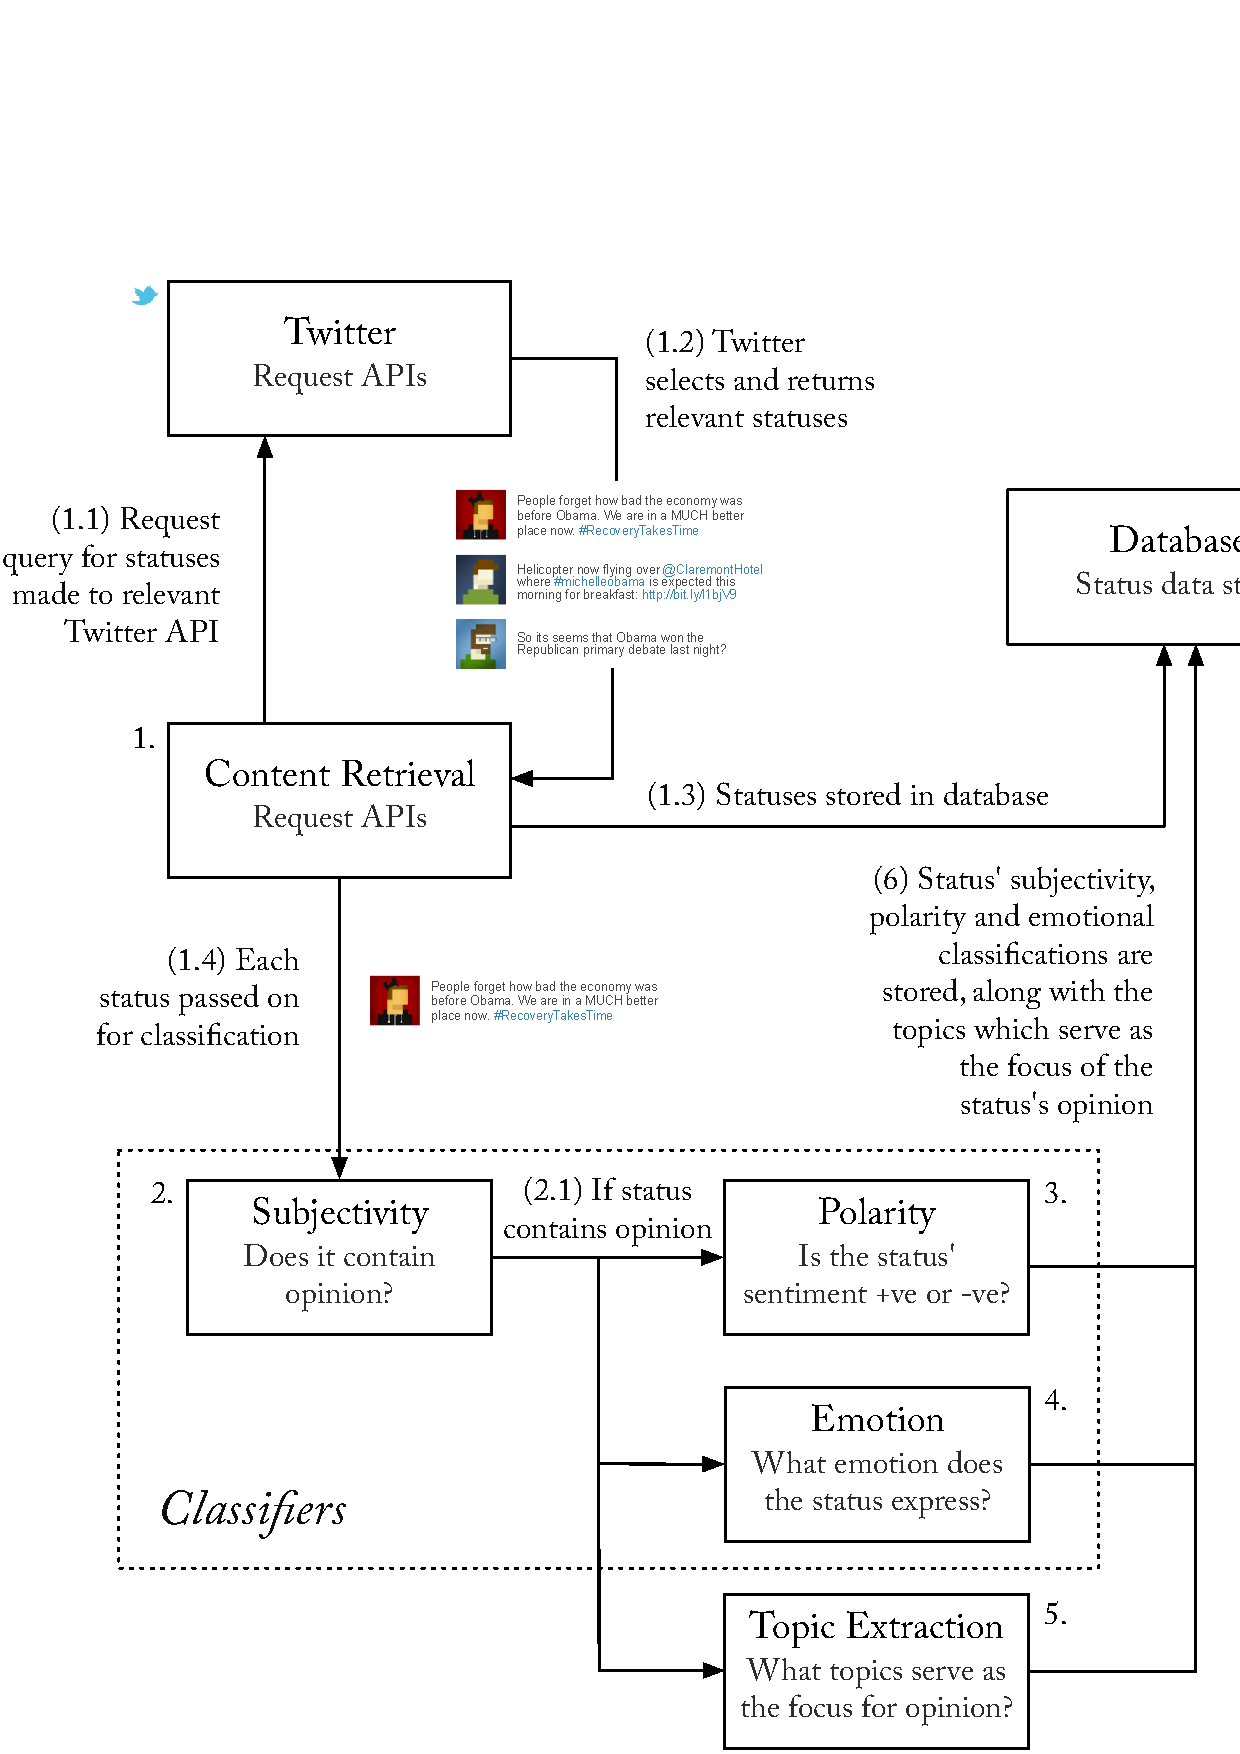
\includegraphics[width=1\textwidth]{figures/outline.pdf}
\end{figure}

We will discuss the first five components in more detail in their own relevant chapters. Classification storage will be referenced where relevant in other chapters, however it does not warrant detailed discussion on its own. 

\section{Implementation narrative}

Throughout our discussion of the project's implementation we shall use five example tweets to help illustrate the classification process within the system. 

\begin{tabular}{ | l | p{4in} | }
	\hline
	No. & Text \\
	\hline
	1. & I think David Cameron is doing a rather good job: strong leader, holding together seemingly impossible coalition, keeping labour at bay \\ %(4dfba78ea590e5055600074f)
	2. & BBC Obama, Merkel warn on Europe debt http://bbc.in/jfZW3I \\ %(4dee52e297dee90936000312)
	3. & \#Obama says European debt crisis can't be allowed to threaten global economy. Shame US never felt this way about its financial crisis. \\ %(4dee52e297dee90936000310)
	\hline
\end{tabular}






	
	\chapter{Content retrieval}
\label{retrieval}

In order to analyse sentiment on Twitter, the first problem posed is how exactly we retrieve the necessary data for analysis. In essence there are two types of data we need, Twitter data for labelling in order to train our system and a much larger set of Twitter data to classify, in order to better understand sentiment on Twitter. We will draw these two slightly disparate elements together under the banner of content retrieval, as although their intended use is quite different, the two types of data share many similarities both in the way they are collected and stored. Once collected the data must then be prepared either for training or classification. This chapter shall first examine the Twitter APIs relevant to this project along with how they are accessed and used. It will then go on to discuss any pre-processing which takes place, before going on to discuss how we label and annotate our data. Lastly we shall evaluate the success of the system in our evaluation section.

\section{Data structure and storage}
\label{retrieval:data}

As described above, information regarding statuses\footnote{We will use the terms \emph{status} and \emph{tweet} interchangeably throughout this project to refer to the same concept. Not only do Twitter use the term status within their object model, but it is also semantically more accurate for this project which eventually hopes to classify statuses from a variety of micro-blogging services.} serves two purposes within this project, firstly when labelled it can serve as training data, and if unlabelled, it can be classified by our sentiment analysis engine in the hope of better understanding the overall opinion and emotion on Twitter. Essentially this means that every status retrieved can be expanded upon with additional information pertaining to both an annotator and-or classifier's decisions as to its sentiment labels. Throughout this project we shall use MongoDB as our primary data store, both for reasons we shall give throughout the rest of this chapter and those outlined in chapter \ref{background}. Although MongoDB does not require that documents added to it adhere to any schema, the requirements of our project insist that the basic attributes illustrated in listing \ref{retrieval:example_json_tweet} are present. Both \texttt{trained\-\_status} and \texttt{classified\-\_status} are optional additional attributes.

\begin{lstlisting}[language=Ruby, caption={Basic JSON structure for status objects stored in MongoDB}, label=retrieval:example_json_tweet]
{
	"text" : "Hi, this is an example tweet!"
	"source" : "search_api" | "streaming_api"
	"source_id" : NumberLong("78133750344597504"),
	"posted_at" : "Tue Jun 07 2011 17:18:46 GMT+0100 (BST)",
	"from_user" : "joeroot"
	"trained_status" : {
		"subjectivity" : "subjective" | "objective" | "spam"
		"polarity" : "positive" | "negative" | "neutral"
	}
	"classified_status" : {
		"subjectivity" : "subjective" | "objective" | "spam"
		"polarity" : "positive" | "negative" | "neutral"
	}
}
\end{lstlisting}

In order to express this JSON structure within Ruby, we will create three new classes, \emph{Status}, \emph{TrainedStatus} and \emph{ClassifiedStatus}. The core status class will consist of all the attributes described within our JSON schema (listing \ref{retrieval:example_json_tweet}), along with attributes for retrieving a \emph{Status}'s relevant training or classification data. Both the \emph{TrainedStatus} and \emph{ClassifiedStatus} classes will maintain the \emph{Status} class' original attributes, along with new ones for accessing any relevant label data. As shown in figure \ref{fig:status_uml}, both \emph{TrainedStatus} and \emph{ClassifiedStatus} inherit attributes from their parent \emph{Status} class.

\begin{figure}[h!]
	\caption{Class structure for representing tweets/statuses}
	\label{fig:status_uml}
	\centering
	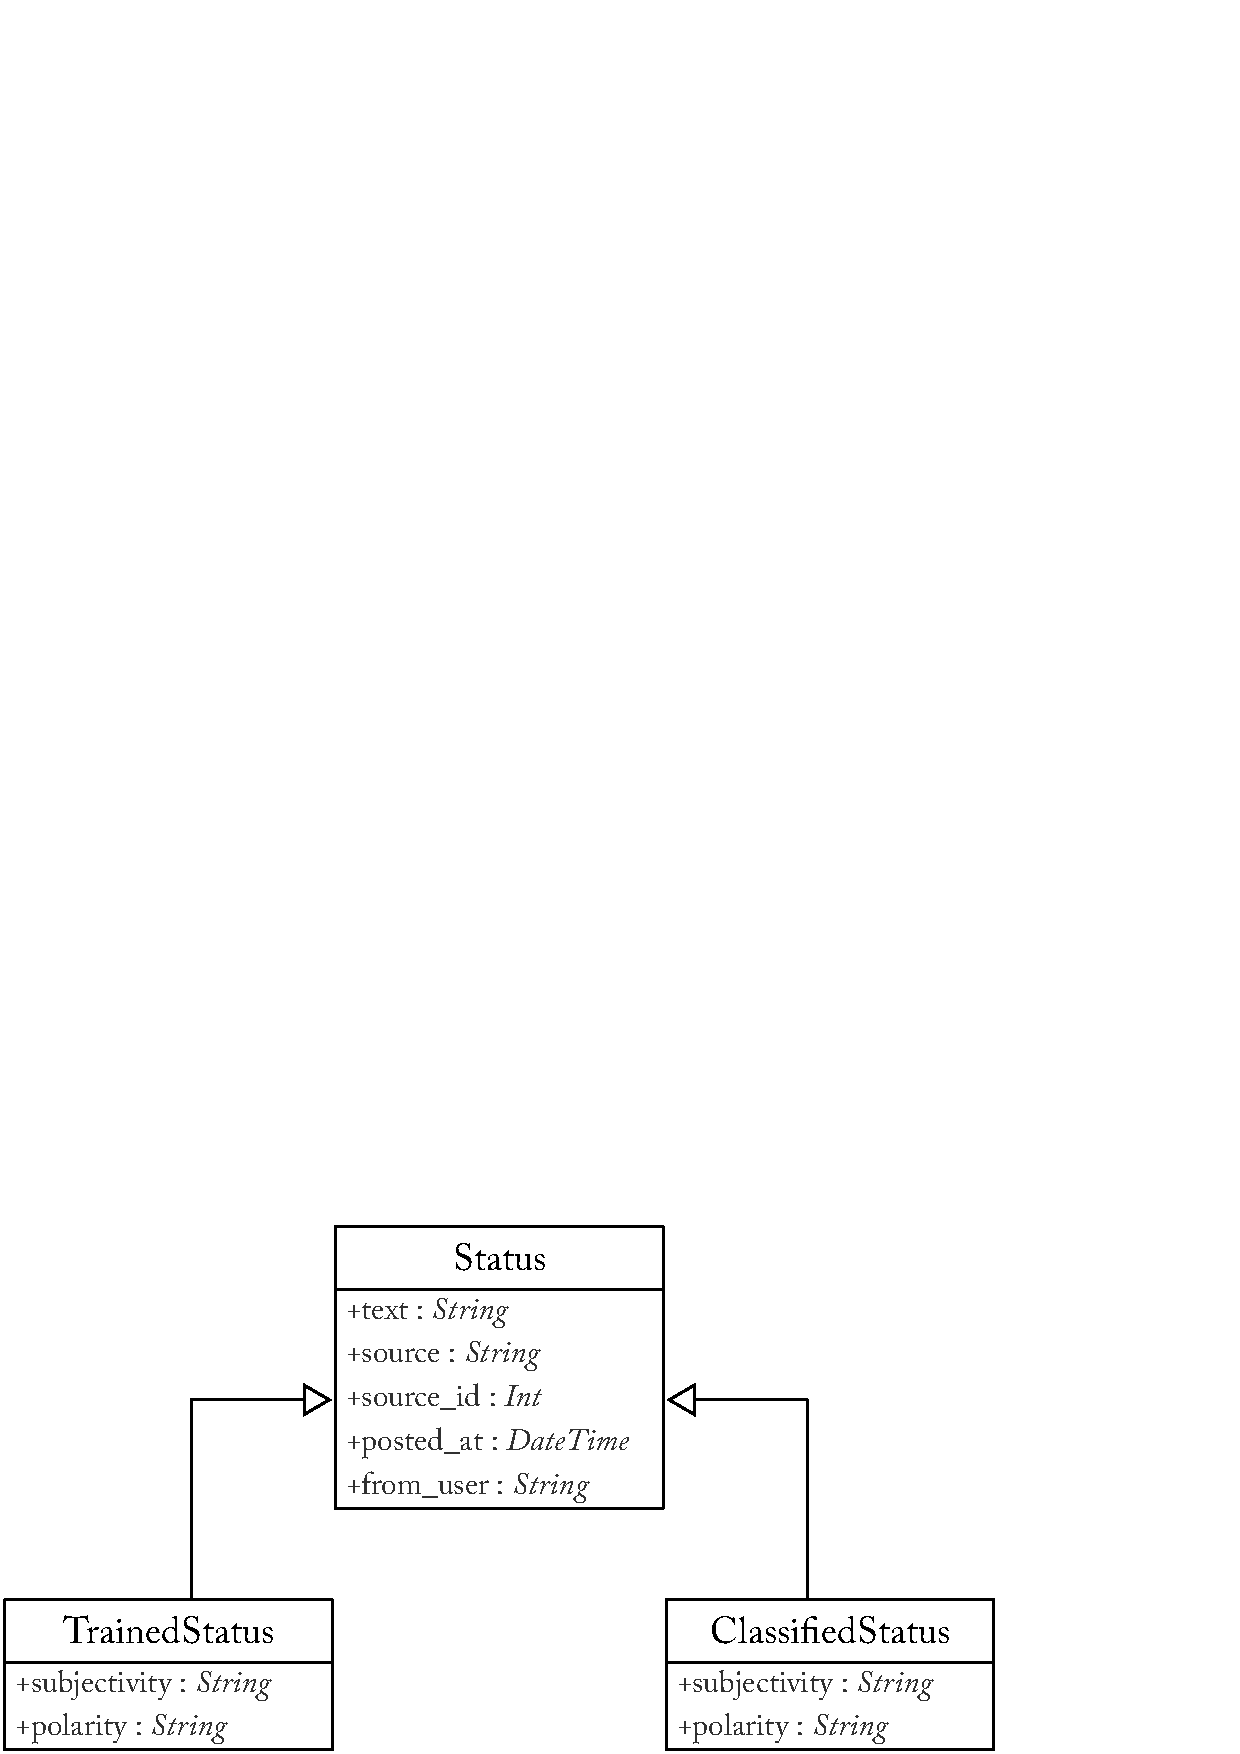
\includegraphics[width=0.83\textwidth]{figures/status_uml_class_diagram.pdf}
\end{figure}

As we go on to explore other components in later chapters, we will add and expand upon this initial core set of attributes and methods. 

The simplicity of MongoDB means any additional data which might be discovered regarding tweets can be inserted as new attributes without any schema worries. In order to map our MongoDB data to Ruby classes we have used an open-source library called \emph{MongoMapper}. MongoMapper gives us the ability to map class objects and attributes to documents within MongoDB. This means that rather than loading and storing an object's attributes in memory, MongoMapper will always read and write directly to the relevant database document. Listing \ref{retrieval:status_code} demonstrates how this mapping is setup for the \emph{Status} class.

\section{Retrieving content on Twitter}

Twitter offers three core APIs for accessing their data, all of which return the said data in either JSON or ATOM format. The three APIs offered are:

\begin{description}
	\item [REST API] - Twitter's REST API provides direct access to Twitter's data model. Requests can be made to access a wide variety of Twitter data, such as user information, timelines, statuses and trends. Essentially Twitter makes all of their sites functionality available through it's API.
	\item [Search API] - Twitter's search API makes their internal status search engine available to developers. Given a query and set of parameters, the search API will find all relevant statuses and return them in the requested format. The status objects returned contain less information than those in the REST API.
	\item [Streaming API] - Twitter's streaming API grants developers access to a high-throughput near-realtime percentage of Twitter's live data. In general Twitter makes 1\% to 10\% of all statuses available through the API and includes further methods for filtering by keywords.
\end{description}

This project shall make use of the \emph{search} and \emph{streaming} APIs. The search API will be used to find tweets for labelling whilst the streaming API shall be employed to collect and filter data for classification. As noted in section \ref{retrieval:data}, data is stored in MongoDB as JSON objects, thus all API calls will request that results be returned in JSON.

\subsection{Search API}

Twitter's search API allows developers to search for tweets matching a specified set of criteria. This is made available through a web-based API, accessible by making GET requests to \texttt{http://\-search\-.\-twitter\-.\-com\-/\-search\-.\-json}. Parameters can be passed to the API through the request headers. For example appending \texttt{q=\-david\-\%20cameron} to the request headers would prompt the API to search for all statuses containing the words "david" and "cameron". Twitter formats the returned data as JSON, with the search results being stored as an array of tweets in the \texttt{results} variable, as demonstrated in listing \ref{retrieval:example_search}.

In order to search and store Twitter data, we created a singleton \emph{TwitterSearch} class. It's \texttt{search} method takes a query string and a parameters hash\footnote{It is common practise amongst Ruby developers to use a \emph{parameters hash} for passing in optional methods to a method. The hash is declared last in a method's arguments, and can be left out when calling the method. If left out, the method definition ensures that the parameters hash is instantiated as an empty hash to prevent any \texttt{nil} errors.}. The parameters hash is used to pass in optional arguments, which map directly to Twitter's search API's optional arguments. Optional parameters include restricting tweets to certain languages through the \texttt{locale} parameter or the \texttt{until} parameter for finding tweets up to a specified date. The query string and parameters are then combined to generate a request URL. Once generated, the \texttt{open-uri} library is used to make a GET request to the URL, and the returned JSON data is stored in a local variable for formatting. Each result's JSON data is amended with a \texttt{source} attribute to identify that the status was retrieved using the Twitter search API. The remaining JSON data however is left unchanged and intact. Once amended, each result is initialised as a \emph{Status} object using it's JSON data. When initialised, MongoMapper automatically writes the data to MongoDB for later use, thus all results are persisted within our database.

Although there are plenty of Ruby libraries available for accessing Twitter's search API, they are often bloated. Many implement their own class structure for representing Twitter's object model which is both unhelpful and unnecessary for this project. Furthermore, although some offer cacheing, none provide support for database persistence. Instead our choice of MongoDB and MongoMapper mean that simply through retrieving the JSON results and using them to initialise \emph{Status} objects, we will have persistent access to the results. 

\subsection{Streaming API}

Twitter's graded streaming APIs deliver developers realtime Twitter data. The three grades, \emph{spritzer}, \emph{garden-hose} and \emph{fire-hose} offer different volumes, ranging from 1\% to 100\% of all realtime tweets. This project shall utilise the \emph{garden-hose} level, which delivers between 1\% and 10\% of all live statuses. Furthermore Twitter offer API methods for filtering the stream ensuring that only tweets matching an array of keywords are included. Twitter make this available by opening an HTTP connection, but never closing it. Tweets are then passed down this connection to the developer. The method call is made to \texttt{http://\-stream\-.twitter\-.com\-/1\-/statuses\-/fi\-l\-ter\-.json} using the \texttt{track} parameter to pass in the set of keywords. For example appending \texttt{track=nhs,david\%20cameron} to the request header will filter the stream for all tweets containing "nhs" or "david cameron". The results are formatted as JSON with each result being separated by a line break. The returned data is slightly more detailed than that returned by the search API, however the core data still adheres to the same schema.

\section{Pre-processing}
\label{subjectivity:pre-processing}

Pre-processing hopes to determine the linguistic attributes of a status which have not already been computationally identified. Primarily we are interested in identifying any grammatical meta-data, in this case each word's part of speech tag, along with any Twitter meta-data the word might contain such as hashtags and mentions. Although not necessarily features themselves, this additional detail will help better describe the data and thus prove useful when building features which truly understand the linguistic nature of Twitter statuses.

\subsection{Part of speech tagger}

Numerous approaches have been taken to part-of-speech tagging, however for the purpose of this project we will implement a Ruby adaptation of Coburn's Perl part of speech tagger\footnote{http\-://\-search\-.cpan\-.org\-/~\-acoburn\-/Lingua\--EN\--Tagger}. Coburn's approach is dependant upon a large corpora of text, within which each word has been annotated with its part of speech tag. For each word within the corpora, we calculate the probability of it being used as a certain part of speech, given by how often it occurs as that said part of speech. For example, if the word \emph{like} appears twice as a an infinitive verb, and once as a past tense verb, the probability of it being an infinitive verb will be $\frac{2}{3}$, and the probability of it being a past tense verb will be $\frac{1}{3}$.

\begin{equation}
	\Pr(tag \mid word) = \frac{|\occurences(word \text{ as } tag)|}{|\occurences(word)|}
\end{equation}

Once this is done, we then use the corpora to calculate the probability of a tag occurring, given the previous word's tag. For example, if an infinitive verb is followed by a proper noun twice and an adjective once, then the probability of a word being a proper noun given the word before it was an infinitive verb is $\frac{2}{3}$, and the probability of it being an adjective is $\frac{1}{3}$.

\begin{equation}
	\Pr(tag \mid tag_{p}) = \frac{|\occurences(tag_{p} \text{ preceeding } tag)|}{|\occurences(tag_p)|}
\end{equation}

Thus, when determining a word's part of speech tag, we want to find the tag which maximises the product of the two probabilities, given our current word and the part of speech tag for the word which preceded it.

\begin{equation}
	\label{eqn:pos}
	\pos(word,tag_{p}) = \argmax_{tag \in tags} (\Pr(tag \mid word) \cdot \Pr(tag \mid tag_{p}))
\end{equation}

Our \emph{TweetTagger} class replicates the above behaviour in Ruby. Colburn's pre-trained probabilities are stored in two separate text files and read into two hashmaps when a \emph{TweetTagger} object is instantiated. In order to tag a body of text with it's appropriate part of speech tags, we can call the \texttt{fetch\_tags(text)} method, passing in the body of text we wish to tag as a parameter. Before we tag the text, it is first split on it's white space and punctuation, using our \texttt{split(text)} function, as demonstrated in listing \ref{overview:example_split_function}.

\begin{lstlisting}[language=Ruby, numbers=none, caption={Example use of split function}, label=overview:example_split_function]
TweetTagger.new.split("Hello, please split this string.")
	=> ["Hello", ",", "please", "split", "this", "string", "."]
\end{lstlisting}

Once split, we are able to tag each word and punctuation mark with it's appropriate part of speech tag. This is done through the \texttt{assign\_tag\-(word\-, \-previous\_tag)} method, a Ruby implementation of equation \ref{eqn:pos}. Where a word does not exists within our lexicon of trained probabilities, and thus no probability score can be calculated for it, it is passed on to the \texttt{unknown\_word\-(word)} method. This attempts to find the word elsewhere, and will be of particular use when adapting the tagger for use on Twitter statuses, and is discussed in detail in section \ref{retrieval:pos_statuses}. For now however, we will assume it manages to find the correct tag.

Once every word has been tagged, the \texttt{fetch\_tags(text)} method returns a JSON formatted, ordered array of words and their corresponding tags. For example, if we were to call \texttt{fetch\_tags} with \emph{Example 1}, the returned JSON would be as shown in listing \ref{overview:example_1_pos_json}.

\begin{lstlisting}[language=Ruby, numbers=none, caption={Returned part of speech tags for \emph{Example 1}}, label=overview:example_1_pos_json]
TweetTagger.new.fetch_tags("I think David Cameron is doing a rather good job: strong leader, holding together seemingly impossible coalition, keeping labour at bay")
	=>	[{"word" : "I", "tag" : "prp"}, {"word" : "think", "tag" : "vbp"}, {"word" : "David", "tag" : "nnp"}, {"word" : "Cameron", "tag" : "nnp"}, {"word" : "is", "tag" : "vbz"}, {"word" : "doing", "tag" : "vbg"}, {"word" : "a", "tag" : "det"}, {"word" : "rather", "tag" : "rb"}, {"word" : "good", "tag" : "jj"}, {"word" : "job", "tag" : "nn"}, {"word" : ":", "tag" : "pps"}, {"word" : "strong", "tag" : "jj"}, {"word" : "leader", "tag" : "nn"}, {"word" : ",", "tag" : "ppc"}, {"word" : "holding", "tag" : "vbg"}, {"word" : "together", "tag" : "rb"}, {"word" : "seemingly", "tag" : "rb"}, {"word" : "impossible", "tag" : "jj"}, {"word" : "coalition", "tag" : "nn"}, {"word" : ",", "tag" : "ppc"}, {"word" : "keeping", "tag" : "vbg"}, {"word" : "labour", "tag" : "nn"}, {"word" : "at", "tag" : "in"}, {"word" : "bay", "tag" : "nn"}]
\end{lstlisting}

Our implementation of Colburn's part of speech tagger proves both fast and accurate on spell-checked bodies of text. However, it performs less well when confronted with the abbreviations, acronyms and mis-spellings common amongst Twitter statuses. Furthermore, it fails to account for Twitter protocols such as hashtags and mentions. It is these issues we will confront in our next section, \ref{retrieval:statuses}.

\subsection{Tagging Twitter statuses}
\label{subjectivity:statuses}

This section shall examine the improvements and additions we have made to Colburn's original tagger, in order to better suit it to the task of tagging Twitter statuses.

\subsubsection{URLs}
\label{subjectivity:urls}

URLs are frequently used within tweets, however Colburn's original design provides no mechanism for handling or tagging them. In order to account for this we decided to introduce an additional \emph{URL} tag to the Penn tag-set along with amending our original tagger to both identify and tag URLs.

But how does this fit into out \emph{TweetTagger} class? As discussed in the previous section, any words which cannot be found in the lexicon are passed on to the \texttt{unknown\-\_word\-(word)} method. Typically this is used to pick up words representing ordinal and float numbers which are not included in the word-probability lexicon. If the unknown word is not a number, other identifiers are examined, such as it's suffix, in the hope that they might provide additional clues for identifying the word's POS. For example, words suffixed with "\emph{ly}" tend to be adverbs or adjectives, thus if the actual word cannot be found in the word-probability lexicon, we assign it probabilities based upon all words ending in "\emph{ly}". In order to match unknown words to their most appropriate identity, such as a number or suffixed word, each word is compared against a regular expression\footnote{Explain regular expressions} corresponding to a potential identity through a series of \emph{if-else} statements. Statements higher up the list take priority, thus for identities which provide certainty, such as numbers, we place their condition higher up the \emph{if-else} chain. In order to help better illustrate this, example code from the method itself is included in listing \ref{overview:example_unknown_function}.

\begin{lstlisting}[language=Ruby, caption={Example if-else statements for handling unknown words}, label=overview:example_unknown_function]
def classify_unknown_word(word)
	if /-?(?:\d+(?:\.\d*)?|\.\d+)\z/ =- word 
	  classified = "*NUM*"	# Floating point number
	elsif /\A\d+[\d\/:-]+\d\z/ =- word  
	  classified = "*NUM*"	# Other number constructs
	elsif /\A-?\d+\w+\z/o =- word
	  classified = "*ORD*"	# Ordinal number
	elsif
		...
	end
	return classified
end
\end{lstlisting}

In order to determine whether a word is in fact a URL, an additional condition is added to the \texttt{unknown\_word(word)} method in order to  check whether it matches against our URL regular expression (see table \ref{table:regex}). With the tagger now amended, if a tweet containing a URL is passed in, the URL is split off into it's own word and tagged as a URL, as demonstrated in listing \ref{overview:example_url_function}. Finally it is important to note that as we have now introduced a URL tag, we need to introduce a probability set for words following our new tag within the \emph{tag-probability} lexicon. The new entry into the lexicon is used for calculating the most appropriate tags for any word directly following a URL. URLs are typically used as nouns when not at the end of sentences, thus rather than rebuilding our lexicons with a small corpora of tweets, we chose to simply assign the same next tag probabilities to URLs as we have for nouns.

\begin{lstlisting}[language=Ruby, numbers=none, caption={Example use of split function}, label=overview:example_url_function]
TweetTagger.new.fetch_tags("BBC Obama, Merkel warn on Europe debt http://bbc.in/jfZW3I")
	=>[{"word" : "BBC", "tag" : "nnp"}, {"word" : "Obama", "tag" : "nnp"}, {"word" : ",", "tag" : "ppc"}, {"word" : "Merkel", "tag" : "nnp"}, {"word" : "warn", "tag" : "vbp"}, {"word" : "on", "tag" : "in"}, {"word" : "Europe", "tag" : "nnp"}, {"word" : "debt", "tag" : "nn"}, {"word" : "http://bbc.in/jfZW3I", "tag" : "url"}] 
\end{lstlisting}

\subsubsection{Mentions}

As with URLs, mentions are not handled by our initial implementation of Colburn's tagger. Mentions represent a unique entity, thus rather than needing a new tag, they are and can be tagged as proper nouns. Essentially they are used as replacements for names therefore this is both a natural and correct assumption to make. Although we decided to tag mentions as proper nouns, we also wanted to design a way of acknowledging that the word additionally contains Twitter meta-data. In order to do this we decided to expand upon our initial JSON representation to include a \emph{meta} object for each word. Within this meta object we are then able to include additional Twitter data, and in the case of mentions, this is done with a boolean attribute, \texttt{mention}, to denote whether the word is being used as a Twitter mention, as in listing \ref{overview:example_mention_schema}.

\begin{lstlisting}[language=Ruby, numbers=none, caption={Example JSON structure for representing a mention word}, label=overview:example_mention_schema]
{
	"word" : "@BBC", 
	"tag" : "nnp",
	"meta" : {"mention" : true}
}
\end{lstlisting}

Our approach to identifying mentions is similar to that used for URLs. As no word beginning with "@" exist within our lexicon, it is safe to assume all mentions will be passed on to the \texttt{unknown\_word(word)} method. Within this method, an additional condition is added for identifying words which are mentions. The word is accordingly tagged as a proper noun, and it's meta object's mention attribute is set to true.

\subsubsection{Hashtags}

As with mentions, although hashtags are not directly supported by our tagger implementation, they do not require their own part of speech tag. Instead if processed correctly, they can often be tagged as words with a corresponding natural part of speech. Frequently users will amend keywords within their statuses as hashtags without interrupting the flow of the status. This can be seen in \emph{example 3} with the opening word, "\#Obama". Furthermore hashtags are often used to express opinion, for example "\#hate" is an extremely popular hashtag for expressing intense dislike for a status' target. Evidently, understanding a hashtag's genuine part of speech is important if we hope to truly determing its sentiment.

The \emph{TweetTagger} class approaches this by first ammeding all hashtag-words' \texttt{meta} object. This is done by setting the \texttt{meta} object's \emph{hashtag} attribute to true and it's \emph{original} attribute to the actual hashtag-word. Once this is done the hashtag is stripped of it's opening hash, and the word is classified as per usual. For example, in the case of "\#Obama", we would see the corresponding representation as in listing \ref{overview:example_hashtag_schema}.

\begin{lstlisting}[language=Ruby, numbers=none, caption={Example JSON structure for representing a hashtag word}, label=overview:example_hashtag_schema]
{
	"word" : "Obama", 
	"tag" : "nnp",
	"meta" : {
		"mention" : false
		"hashtag" : true
		"original" : "#Obama"
	}
}
\end{lstlisting}

As with both URLs and mentions, this is achieved by adding an additional condition to the \texttt{unknown\_word(word)} method. Unlike with mentions and URLs however, the word is stripped of it's opening hashtag, and passed back for retagging. This enables us to find its genuine part of speech tag by observing its position within the status text.

\subsubsection{Names, misspelling and acronyms}

\section{Labelling data}
\label{retrieval:labelling}

The primary use of our search API interface, \emph{TwitterSearch}, is to ease the process of collecting data for labelling. Rather than doing this within code, it was deemed simpler and quicker to build a web-based interface for searching and classifying tweets. The interface is built using a combination of HTML, CSS and JavaScript for the front-end, whilst the back-end data management is handled by a Ruby web-framework, Sinatra.



	\chapter{Classifiers}
\label{classifiers}

At the heart of this project's sentiment analysis lie our three classifiers for subjectivity, polarity and emotion. For reasons we shall discuss in their respective chapters, we have elected to take either a supervised or semi-supervised approach to learning for all three classifiers. As a result, our classifiers' implementations share much in common. In particular, this chapter shall focus on how this commonality can be unified through our \emph{Classifier} class. This project is largely experimental in nature, looking at how we can best adapt, use and develop existing and new ideas for classifying sentiment on Twitter. As a result, we wanted to design a parent \emph{Classifier} class which would best remove the  complexities of correctly assembling and training our classifiers. We wanted a class which would allow us to focus on experimenting with different feature sets and classification techniques, along with providing tools for gathering and comparing our results. The remainder of this chapter shall first outline our core aims for the class, before going on to discuss our approach. After this we will summarise the methods discussed and implemented within our class, before finally evaluating overall performance against our original aims.

\section{Overview}
\label{overview}

As discussed above, our \emph{Classifier} class hopes to unify the overall approach taken to classification across the three classifiers. In doing so it hopes not only to save time by eradicating repetition, but also simplify and encourage experimentation through intelligent design. The three core aims of the class are:

\begin{enumerate}
	\item \emph{Simple feature selection} when initialising a classifier. For example, we might want to initialise a classifier with just \emph{feature one} before initialising another classifier for a performance comparison, with both \emph{feature one} and \emph{feature two}.
	\item \emph{Simple classifier method selection} when initialising a classifier. For example we may want to compare the performance of our classifiers when using a Support Vector Machine against using a Naive Bayes classifier.
	\item \emph{Unified testing} for classifiers in which key machine learning metrics such as accuracy, recall, precision and f-measure are automatically calculated. This will ease in comparing and contrasting results for changes in feature set and classification method.
\end{enumerate}

\section{Preparing the data}
\label{classifiers:preparing_data}

In order to train our classifier, we first need to prepare our \emph{training data} accordingly. This means building a feature set for our training data, according to both the \emph{features} we want to use, and the \emph{label} with which we are looking to classify statuses, as explained in figure \ref{fig:building_feature_set}.

\begin{figure}[h!]
	\caption{Outline for building feature set}
	\label{fig:building_feature_set}
	\centering
		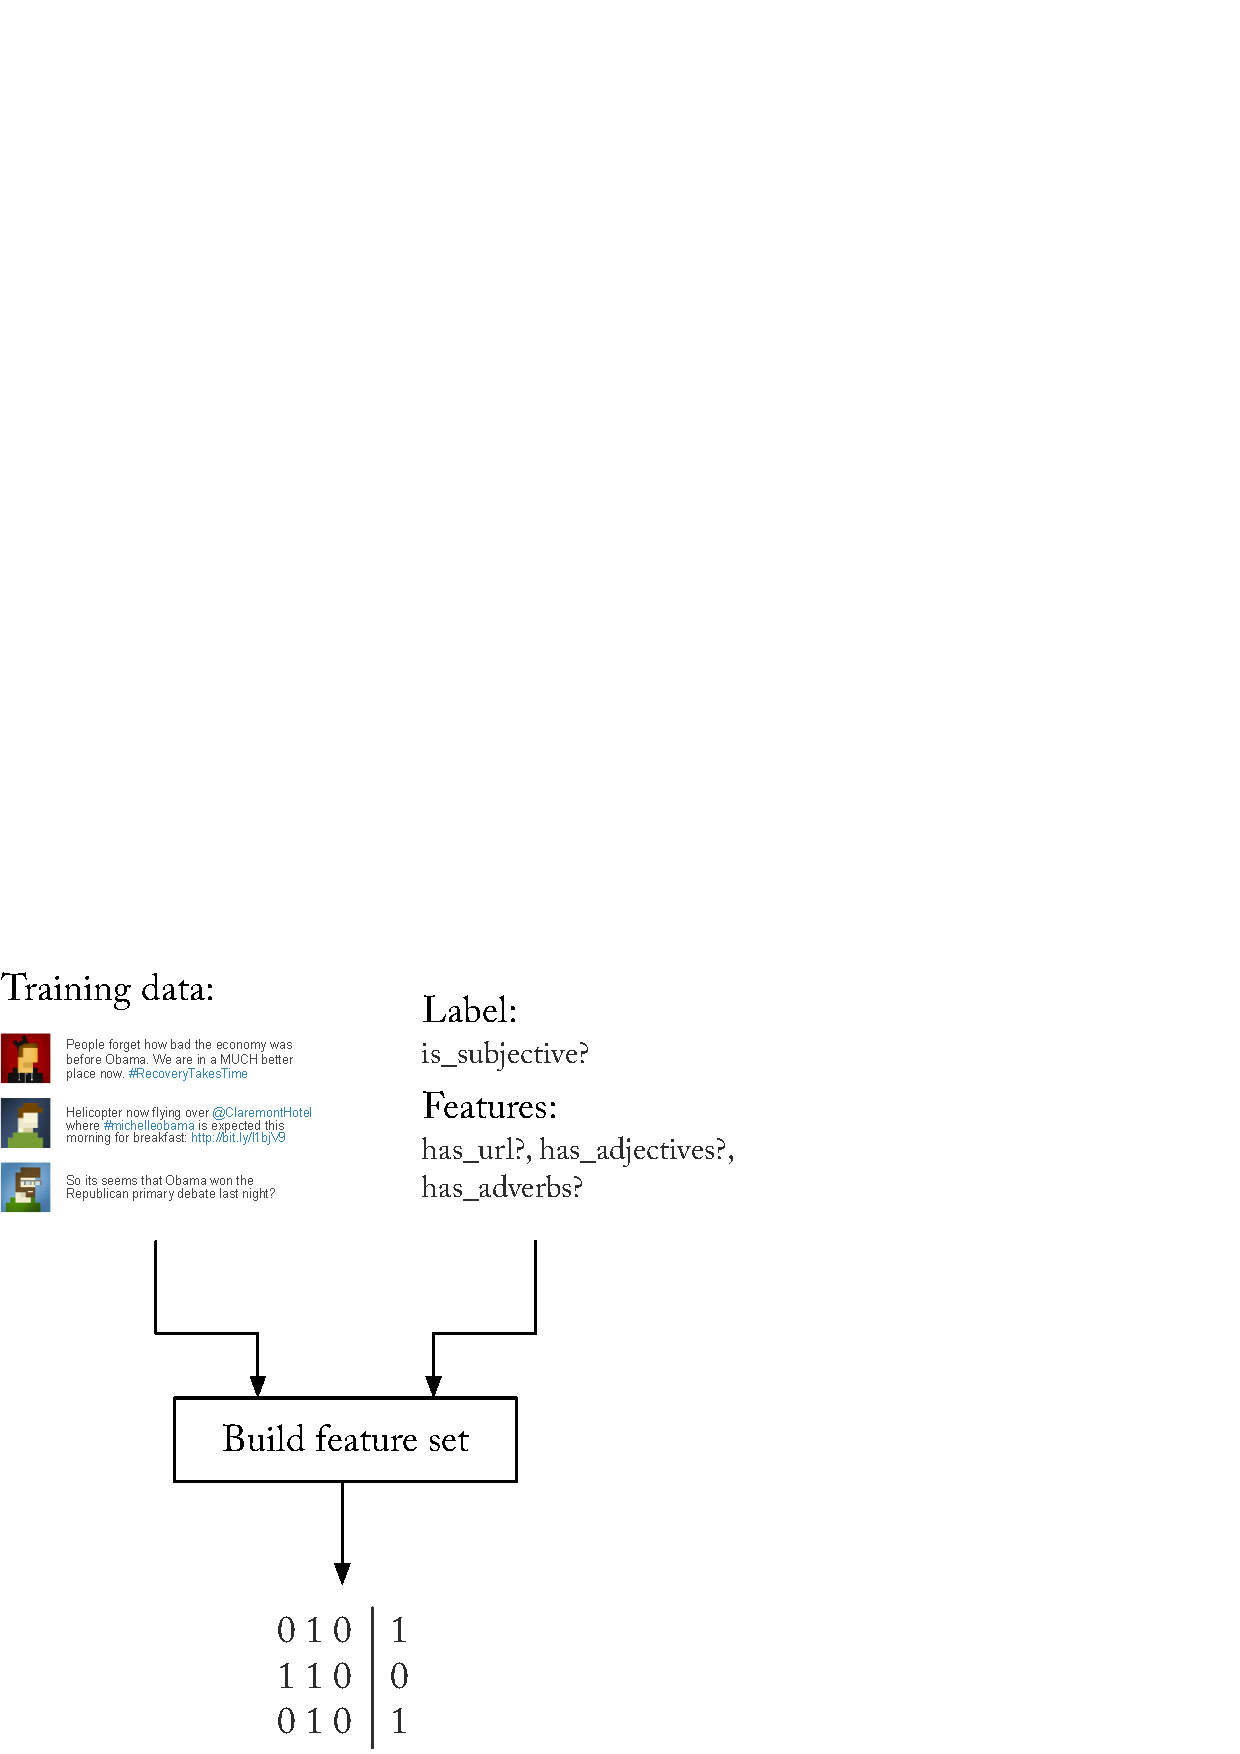
\includegraphics[width=0.6\textwidth]{figures/build_training_data.pdf}
\end{figure}

We wanted our approach to this to be as generic as possible, and in doing so made use of Ruby's \texttt{send} method. Every object within Ruby has a \texttt{send} method which accepts a symbol\footnote{\emph{Symbols} are Ruby's approach to efficient \emph{String} usage. In our case, rather than initialising a new \emph{String} object every time we want to refer to a certain method, a symbol is only very initialised once but can be used throughout our code. Essentially a symbol can be used as a low footprint replacement for \emph{Strings}.} and a series of arguments. When called, Ruby will in turn attempt to call the object's method which corresponds to the given symbol, along with any additional arguments. For example \texttt{"Hello, Joe".send(:split, ", ")} is in effect the same as \texttt{"Hello, Joe".split(", ")} and will return \texttt{["Hello", "Joe"]}. It is this we make use of when trying to take a flexible approach to feature choice. It is important to note that all feature methods take a \emph{Status} object and must be implemented as object level methods within any class extending our \emph{Classifier} class. Thus, using the send method, we can initialise our classifier with an array of symbols representing feature methods, before using this array to generically create our training set, as shown in listing \ref{classifiers:status_feature_set}.

\begin{lstlisting}[language=Ruby, caption={Method for building a status' feature set}, label=classifiers:status_feature_set]
# @features = [:feature\_1,..., :feature\_n]
def build_status_feature_set(status)
	return @features.map{|f| self.send(f, status)}
end
\end{lstlisting}

Given a training set, we simply iterate over it, creating a feature set for each training status. This array of feature sets can now be used to train our classifier.

Before we train our classifier, we also need an array containing each of the training statuses' appropriate label, such as their polarity or subjectivity. It is the values of this label which are classifier will be trained to identify, and just as we defined an array of features to build our feature sets, we will instantiate a single \texttt{label} variable to store the label's method symbol, such as \texttt{:is\_subjective?} or \texttt{polarity}. This is built in a similar manner to our feature sets, using the object \texttt{send} method coupled with the \texttt{label} symbol, and is wrapped up in the \texttt{fetch\-\_status\-\_label\-(status)} method.

\section{Training and classifying}

With our training data now prepared in the form of two arrays, one containing feature sets and one containing labels, we can train our classifier. As explored by Pang et al. \cite{Pang:2008wj}, the classification method used can impact the effectiveness of our results. We decided to experiment with both the leading probabilistic and non-probabilistic methods, these being the \emph{Naive Bayes (NB)} classifier and the \emph{Support Vector Machine (SVM)}. 

Rather than building our own SVM and NB classifiers, we elected to use two well established libraries, LIBSVM and AI4R, as discussed in section \ref{background:tools}. As both utilise their own methods and input schemas for training and classification, we implemented an intermediary interface for both the LIBSVM and the AI4R libraries. Both our \emph{NaiveBayes} and \emph{SupportVectorMachine} classes adhere to this interface, and share the same public methods. Effectively this allows us to initialise both our classifiers using the feature sets and labels generated above, as demonstrated in listing \ref{classifiers:build_classifiers}. 

\begin{lstlisting}[language=Ruby, caption={Example initialisation of LIBSVM and AI4R Naive Bayes classifiers through intermediary layer}, label=classifiers:build_classifiers]
feature_sets = training_statuses.map{|s| self.build_status_feature_set s}
labels = training_statuses.map{|s| self.fetch_status_label s}
svm = SupportVectorMachine.new(feature_sets, labels)
nb = NaiveBayes.new(feature_sets, labels)
\end{lstlisting}

Whenever a class extending our \emph{Classifier} class is initialised, an additional parameter is passed in alongside the features and label, denoting whether to use a SVM or NB classification method. A new classification method is initialised as described above, and stored within the \emph{Classifier} object's \texttt{classifier} variable. Once the \emph{NaiveBayes} and \emph{SupportVectorMachine} layers have been initialised and trained, they can be used to classify statuses through their \texttt{classify(feature\_set)} method. When given a feature set, this method will classify it and return the appropriate label. This enables us to again make use of the \texttt{build\-\_status\-\_feature\-\_set\-(status)} method from within our \emph{Classifier} class, rather than having to generate a feature set in the appropriate format for the specified classifier method. In order to better illustrate the chain of command, we have included the \emph{Classifier} class' \texttt{classify(status)} method in listing \ref{classifiers:classify}.

\begin{lstlisting}[language=Ruby, caption={\emph{Classifier} class' classify method}, label=classifiers:classify]
def classify(status)
	feature_set = self.build_status_feature_set status
	# @classifier is either an initialised SupportVectorMachine or
	# NaiveBayes object. This is instantiated when initialising our
	# Classifier object.
	return @classifier.classify(feature_set) 
end
\end{lstlisting}

With unobtrusive support for different feature sets and classification methods now implemented within our \emph{Classifier} class, we can finally look at the approach taken to performance testing.

\section{Testing}

Due to the project's strong element of experimentation, providing a robust framework for evaluating our classifiers was essential. As is common within both machine learning and sentiment analysis, our four chosen measure of performance are \emph{accuracy}, \emph{precision}, \emph{recall} and \emph{f-measure}. These four metrics combine to give a fairly clear portrait of a classifiers strengths and weaknesses. In order to better explain each measure we shall first introduce four terms commonly used within binary classification:

\begin{description}
	\item [True positives] are the set of of correctly classified documents for the positive label. For example in subjectivity classification, this could be taken to be all statuses correctly classified as subjective.
	\item [True negatives] are the set of correctly classified documents for the negative label. For example in subjectivity classification, this could be taken to be all statuses correctly classified as not subjective.
	\item [False positives] are the set of incorrectly classified documents, who have been labelled positive when they are in fact negative.
	\item [False negatives] are the set of incorrectly classified documents, who have been labelled negative when they are in fact positive.
\end{description}

Using these four definitions, we can now go onto better define our performance measures:

\begin{description}
	\item [Accuracy] is used to measure how many documents have been correctly classified across the entire training set.
	\begin{equation}
		accuracy = \frac{| TP \cup TN |}{| TP \cup FP \cup TN \cup FN |}
	\end{equation}
	\item [Precision] is a measure of how accurate our positively labelled data is. This is done by looking at what fraction of positively labelled data is actually positive.
	\begin{equation}
		precision = \frac{| TP |}{| TP \cup FP |}
	\end{equation}
	\item [Recall] is a measure of how much of our positive data is correctly labelled as positive by the classifier. This is done by looking at what fraction of positive data was correctly labelled.
	\begin{equation}
		recall = \frac{| TP |}{| TP \cup FN |}
	\end{equation}
	\item [F-measure] combines the classifiers precision and recall rates to give an overall measure of accuracy.
	\begin{equation}
		F_1 = 2 \cdot \frac{precision \cdot recall}{precision + recall}
	\end{equation}
\end{description}

With the definitions of our measures in place, we now had to introduce a suitable method for calculating them. The first method, \texttt{test(k,statuses)}, performs \emph{k-fold cross validation} across the labelled \emph{statuses} passed in to the method. Effectively k-fold cross validation divides our labelled statuses up into $k$ partitions, before iterating through them, each time using $(k-1)$ partitions as training data, and $1$ partition as testing data. This is repeated $k$ times, and the average measures across each of the folds are taken as the test's overall measures. In order to ensure that training is not biased, we always keep the number of training examples belonging to each label the same.

Although this proved suitable for binary classification, it is not suitable for multi-class classification. Instead for classification with two or more output labels, the \emph{precision}, \emph{recall} and \emph{f-measure} are returned for each potential label. As \emph{accuracy} is already measured across all labels, there was no need for it's results to be calculated for each indiviudal label. The full implementation details for this can be seen in listing \ref{}.

We felt however that for strenuous testing one test was not enough, and instead a \texttt{repeat\_test(k,statuses,n)} method was introduced. This repeats the \texttt{test(k,statuses)} method $n$ times, before returning the average of the measures across those $n$ repetitions.

\section{Class summary}

Before we evaluate the performance of our classifier, we will give a quick overview of the core methods along with a description of their inputs, outputs and purpose.

\begin{centering}
	\begin{longtable}{| l | p{0.16\textwidth} | p{0.16\textwidth} | p{0.4\textwidth} |}
		\hline
		Method & Arguments & Returns & Description \\
		\hline
		\texttt{initialize} & \texttt{features}, \texttt{label}, \texttt{classifier\_method}, \texttt{statuses} & \texttt{none} & Intialisation method for creating new Classifier objects. Will intialize and train either a SVM or NB classifier, with the specified \texttt{features} and \texttt{label}, using the labelled \texttt{statuses} as training data. \\
		\hline
		\texttt{classify} & \texttt{status} & \texttt{label} & The classify method takes a \texttt{status} object, converts it into the appropriate feature set before using the trained classifier method to classify the feature set and return the appropriate \texttt{label}. \\
		\hline
		\texttt{test} & \texttt{k}, \texttt{statuses} & \texttt{accuracy}, \texttt{precision}, \texttt{recall}, \texttt{f-measure} & Given a set of \texttt{statuses}, will split the data into \texttt{k} folds, before testing and training with each. Returns average \texttt{accuracy}, \texttt{precision}, \texttt{recall} and \texttt{f-measure} across the \texttt{k} folds. \\
		\hline
		\texttt{repeat\_test} & \texttt{k}, \texttt{statuses}, \texttt{n} & \texttt{accuracy}, \texttt{precision}, \texttt{recall}, \texttt{f-measure} & Runs \texttt{test(k, statuses)} \texttt{n} times, returning the average \texttt{accuracy}, \texttt{precision}, \texttt{recall} and \texttt{f-measure} across those \texttt{n} repetitions. \\
		\hline
	\end{longtable}
\end{centering}

\section{Evaluation}

The \emph{Classifier} class proved fundamental within this project both as a class and a tool. It has allowed for the remainder of our implementation to focus on innovative feature use and performance, rather than a struggle for consistency across different classifiers. In order to better evaluate the classifier, we shall examine to what extent it met it's original three aims:

\begin{enumerate}
	\item The approach taken to simple feature switching meant that new ideas could be experimented and developed easily, without having to worry about adapting our code elsewhere.
	\item As with feature selection, the class' ability to swap classification methods was simple and effective. It required no additional work throughout the remainder of the project and made evaluation much simpler.
	\item The strong performance testing suite provided a very simple method for meaningfully comparing features and classification methods. This proved vital in understanding how best to approach feature and method selection, along with being fundamental to our evaluation process.
\end{enumerate}

Although no numeric measure can be given to express the class' performance, the fact that it met each of its original aims and the freedom it gave to focus on innovation and testing clearly made it a success.


	\chapter{Subjectivity classification}
\label{subjectivity}

USE BRILL TAGGER

If using a lexicon, look at it's coverage over the training set, i.e. does each subjective word in the lexicon exist in one or more examples. How many subjective examples do not contain words from the subjective lexicon?
	
	\chapter{Polarity classification}
\label{polarity}

Given that we can now determine whether a status contains an opinion, the next stage within our sentiment analysis engine lies in determining the status' polarity. Polarity classification specifically looks at determining whether a status is \emph{positive}, \emph{negative} or in some cases \emph{neutral}. Approaches to classifying polarity have typically been supervised. This is largely due to the difficulty of identifying the numerous nuanced linguistic details which could imply polarity. Although some \cite{Turney:2002vv} have attempted this un-supervised approach, recent work such as that covered by Liu \cite{Liu:2010tm} has seen far more success when taking a supervised approach. Accordingly, we elected to take a supervised approach for polarity classification, with the hope that we might also be able to draw upon some of the linguistic insight offered by unsupervised approaches.

In this chapter we shall first examine how we labelled and annotated our training set, before going on to explore our choice of potential features and their implementations. Next we shall discuss the results of our testing and explain our choice of features, before finally evaluating the success of our classifier with particular respect to prior research.

% "The PM's 18 week waiting time pledge will not mean any change for how the \#NHS is operating: http://bit.ly/kSjpfL" interesting, how do we know no change is good?

\section{Training set}

\section{Features}

\subsection{Unigrams}

As noted by Pang and Lee \cite{Pang:2002tu}, unigrams can often serve as strong discriminative features when classifying polarity. In effect unigrams provide a presence feature for all possible words, however their implementation means that this set of words is limited to those seen when training the classifier, rather than the actual set of all possible words.

As the implementation for unigrams is so distinct from other features, its feature code was built directly into the \emph{Classifier} class, rather than our \emph{PolarityClassifier} class. In order to build our unigrams, we require a two stage process. Before training occurs our unigram set is initialised by iterating through each status, adding its words to our unigram set.  When added, words' are down-cased in order to avoid adding the same word multiple times. Once finished we have an array consisting of very single word used in all of our training examples.

When building a status' feature set either for training or classification, we make use of the previously built array of unigram words. For every word in the unigram array, a feature is added to the status' feature set denoting whether that word occurs within the status. In order to do this we built a \texttt{parse\_unigram(status)} method, which when given a status, will return the corresponding unigram feature set, as shown in listing \ref{polarity:unigrams}.

\begin{lstlisting}[language=Ruby, caption={Example feature set}, label=polarity:unigrams]
def parse_unigrams status
	# downcases and collects every word within the status
  words = status.parts_of_speech.map{|p| p["word"].downcase}
	# iterates over the array of unigram words, noting whether the unigram exists within our status' set of words 
  self.unigrams.map{|u| words.include?(u) ? 1 : 0}
end
\end{lstlisting}

Alongside the \texttt{parse\-\_unigram\-(status)} method, we introduced two other methods. The \texttt{parse\-\_hashtag\-\_unigram\-(status)} produces a unigram feature set in which only hashtags are used as unigrams feature. An additional, more detailed method, \texttt{parse\-\_pos\-\_unigram\-(status)} creates a feature for every word and part of speech tag combination.

In order to simplify the process of including unigrams in our feature set, our classifiers can be initialised with any combination of the three unigram-based features below, just as we would with a normal features. If any of them are included, their corresponding method is called, and its resultant feature set is added to the status' overall feature set. These three methods are:

\begin{description}
	\item [\texttt{unigrams}] is our primary unigram feature. It calls the \texttt{parse\-\_unigram\-(status)} for each status, and appends the resultant feature set to the status' overall feature set.
	\item [\texttt{hashtag\_unigrams}] builds a unigram feature set using only hashtags rather than all word. It calls the \texttt{parse\-\_hashtag\-\_unigram\-(status)} for each status, and appends the resultant feature set to the status' overall feature set.
	\item [\texttt{unigrams\_pos}] builds a more specific unigram feature set than \texttt{unigrams} in which a unigram is only present if both the word and part of speech it represents occur within the status. It calls the \texttt{parse\-\_pos\-\_unigram\-(status)} for each status, and appends the resultant feature set to the status' overall feature set.
\end{description}

In order to help clarify how the \texttt{parse\-\_unigram\-(status)} method works, an example has been given in listing \ref{polarity:unigram_output}.

\begin{lstlisting}[language=Ruby, caption={Unigram parsing for \emph{Example 1} using a small unigram set}, label=polarity:unigram_output]
# let status = Example 1
# let self.unigrams = [think, hate, love, good, bad, strong, weak]
parse_unigrams status
	=> [1,0,0,1,0,1,0]
\end{lstlisting}

\subsection{Polarity clues}
\label{polarity:clues}

Polarity clues are used to identify terms which express polarised opinion. This is a core feature of most polarity classifiers, although the approaches to determining whether a word is polarised vary. We will again draw upon the work of Wiebe and Riloff \cite{Wiebe:2003wa} using chapter \ref{subjectivity}'s \emph{ClueFinder} class. In addition to using the polarised clues presented by Wiebe and Riloff, we also use our own annotated collection of clues and seed words by additionally loading them into the lexicon.

Furthermore when finding clues within a status we also look to further populate our lexicon. All adjective-conjunct-adjective trigrams are extracted, and if one of the adjectives is contained within our clue lexicon, the other is also added. If the conjunct is "\emph{and}", then the new clue is tagged with the same polarity as the existing clue, and if the conjunct used is "\emph{but}" the new clue's polarity is set to the opposite of the existing clue's. Using this un-supervised technique, we are able to further populate our lexicon with no additional effort. This is run on all input statuses, thus it is assumed that the lexicon will improve with time. 

Using our \emph{ClueFiner}'s original \texttt{clue\_data} method we define an additional four methods for our \emph{Status} object, \texttt{weak\-\_positive\-\_clues}, \texttt{strong\-\_positive\-\_clues}, \texttt{weak\-\_negative\-\_clues} and \texttt{strong\-\_negative\-\_clues}. Each of these are then used to help define twelve new clue-based feature methods. We will define the first four, with the last eight being derivatives which introduce the concepts of \emph{weak} and \emph{strong} clues.

\begin{description}
	\item [\texttt{has\_positive\_clues?}] returns a boolean value denoting the presence of one or more positive clues.
	\item [\texttt{no\_positive\_clues}] returns one of three values based upon the number of positive clues. For zero clues, \texttt{0} is returned, for one or two clues, \texttt{1} is returned and for three or more clues \texttt{2} is returned.
	\item [\texttt{has\_negative\_clues}?] as with \texttt{has\-\_positive\-\_clues?}, but only noting negative clues.
	\item [\texttt{no\_negative\_clues}] as with \texttt{no\-\_positive\-\_clues}, but only noting negative clues.
\end{description}

\subsection{Subjective patterns}

In Turney's \cite{Turney:2002vv} un-supervised approach, he proposes five grammatical structures for identifying subjective phrases. He suggest that the polarity of these phrases are in turn indicative of their sentence's overall polarity. Although we felt that as an un-supervised approach alone it was not suitable for the project, we decided to explore the possibility of using it as a feature within our supervised classification.

Each of the rules from table \ref{background:patterns} are assembled as items within a \texttt{rules} array. Each rule is encoded as a series of three arrays, the first two contain all possible part of speech which the first two words of the phrase \emph{must} be, whilst the last array contains all the parts of speech which the third word \emph{must not} be, as implemented in lines 2 to 8 of listing \ref{background:patterns}. We use \texttt{nil} instead of a third array when the third word can take on any part of speech. With a rule structure now in place, we can split our status into its individual trigrams. Each trigram is then iterated over, each time checking to see if it matches any of the rules expressed in our \texttt{rules} array. Any trigram which matches one of the five rules is added to a \texttt{patterns} array, which is returned upon method completion.

\begin{lstlisting}[language=Ruby, caption={\emph{Status} object method for extracting patterns}, label=polarity:patterns]
def patterns
  rules = [
    [["jj"], ["nn","nns"], nil],
    [["rb","rbr","rbs"], ["jj"], ["nn","nns"]],
    [["jj"], ["jj"], ["nn","nns"]],
    [["nn","nns"], ["jj"], ["nn","nns"]],
    [["rb","rbr","rbs"], ["vb","vbd","vbn","vbg"], nil]
  ]
  
  pos = self.parts_of_speech
  trigrams = (pos + [nil]).each_cons(3).to_a    
  
  patterns = trigrams.select do |first, second, third|
    rules.map do |rule|
      rule[0].include?(first["tag"]) and 
      rule[1].include?(second["tag"]) and 
      (
        !rule[2] or 
        (!third.nil? and !rule[2].include?(third["tag"]))
      )
    end.inject(false){|m,n| m or n}
  end
  
  return patterns
end
\end{lstlisting}

Once our patterns have been extracted we can then look for clues pertaining to their polarity. This is done by using the \emph{ClueFinder} class to determine if the first two word to occur in our clue lexicon, and if so what their polarity is. Using this we define two pattern-based features\footnote{As there is typically no more than one pattern in a status, we have opted to use only presence as featured and not a count.}:

\begin{description}
	\item [\texttt{has\_negative\_patterns?}] returns a boolean value denoting the presence of one or more pattern with a negative polarity. 
	
	\item [\texttt{has\_positive\_patterns?}] returns a boolean value denoting the presence of one or more pattern with a positive polarity. 
\end{description}

\section{Results}

\begin{figure}
	\caption{Individual feature accuracy spreads}
	\label{fig:polarity_accuracy}
	\centering
		\includegraphics[width=1.0\textwidth]{graphs/polarity_a.pdf}
\end{figure}

\begin{figure}
	\caption{Individual figure accuracy}
	\label{fig:polarity_precision}
	\centering
		\includegraphics[width=1.0\textwidth]{graphs/polarity_p.pdf}
\end{figure}

\begin{figure}
	\caption{Individual figure accuracy}
	\label{fig:polarity_recall}
	\centering
		\includegraphics[width=1.0\textwidth]{graphs/polarity_r.pdf}
\end{figure}


\section{Evaluation}



	
	\chapter{Emotion classification}
\label{emotion}

With a status' polarity and subjectivity now classified, we can go on to look at what further understanding of a status' sentiment can be gained through classifying its emotion. Rather than taking a supervised approach as often seen in literature \cite{Alm:2005vc}, we will approach our emotion classification through a largely un-supervised approach. As our goal is to gain additional understanding as to a status' sentiment, we felt that a precise approach, with easily justifiable results was more appropriate. Techniques such as that put forward by Yang et al. \cite{Yang:2007wx}, although seemingly accurate, source labelled data for training and testing with no human input. Instead they use emoticons to generate labels which we felt provided significant room for misguided emotion classification. In particular there is no attempt within their work to determine whether the emoticon truly represents the emotion they are ascribing it. Despite this, we will draw upon elements discussed in supervised approaches, especially with regards to the use of WordNet such as in the approach put forward by Alm et al. \cite{Alm:2005vc}. 


Our approach aims to blend aspects of common lexicon-based classification, with the deeper semantic insight gained through the use of tools such as WordNet. Essentially, we hope to determine whether a word and the sense in which it is being used, relate any information to is regarding emotion. As WordNet semantically defines concepts of emotion and feeling, it will prove fundamental in our approach. Within this chapter we shall first briefly examine what exactly WordNet is, before going on to discuss our implementation of it. We shall then go on to explore how exactly we used WordNet to generate our lexicon, before examining how exactly it is used in order to determine any emotion a status might contain. Lastly we shall examine the extent to which our approach was a success along with its potential for any further improvements.

\section{WordNet}
\label{emotion:wordnet}


\section{Building an emotion lexicon}

\section{Classifying emotion}

\section{Evaluation}

	
	\chapter{Topic extraction}
\label{topic}
	
	\chapter{Delivery}
\label{delivery}

With each of our core components now in place, this final chapter hopes to draw all the individual pieces together, along with discussing how they have been made available.

\section{Sentiment analysis engine}

Our sentiment analysis engine is brought together through the singleton \emph{Engine} class. This class initialises each of our three classifiers along with our topic extraction engine. Once initialised, status objects can be classified by calling its \texttt{classify(status)} method, which will return a hashmap containing each of the classifiers' results along with the status' topics, as demonstrated in listing \ref{delivery:classify_results}. The method can handle both \emph{Status} objects and \emph{Strings}.

\begin{lstlisting}[language=Ruby, caption={Returned part of speech tags for \emph{Example 1}}, label=delivery:classify_results]
# let status = Example 1
Engine.classify status
	=>
		{
			:subjective => true,
			:polarity => :positive,
			:emotion => [:trust],
			:topics => ["David Cameron", "job", "leader", "coalition", "labour"]
		}
\end{lstlisting}

Along with returning the results, the hashmap is written as JSON to the status' \texttt{classified\_status} attribute. Thus the above output is persisted in MongoDB and is referred to from that point forward whenever the status' classification is requested.

When the engine is running, it sets the \emph{TwitterStreaming} API to run in the background, constantly feeding data into MongoDB. Our sentiment engine polls this is every 10 seconds checking for new unclassified statuses, and if found it will syphon them off to the \texttt{classify(status)} method.

\section{Online API}

In order for us and others to make use of our collected and classified data, we offer two core web services. Our first, a classification service, is based upon our \emph{Engine} class. The second, a retrieval service, is built upon our MongoDB store. The web services are made available using the \emph{Sinatra} web framework. Below, is a more detailed outline of each service:

\begin{description}
	\item [\texttt{/classify?text=:string}] - when passed a status' textual content, this method will utilise the \emph{Engine} class in order to classify it. The text is formatted as a String object, and passed to the \texttt{classify(status)} method. The returned hashmap is formatted as JSON and delivered back to the user.
	\item [\texttt{/results/:params}] - allows the user to query our MongoDB store for classified statuses. With no parameters, the method will simply return the last 200 classified statuses. With parameters, the user can specify \texttt{from} and \texttt{until} dates to retriever statuses from within a certain time frame. Additionally, the \texttt{subjective}, \texttt{polarity}, \texttt{emotion} and \texttt{topic} parameters each take a comma separated list of acceptable values. For example, 
	\begin{center}
		\texttt{polarity=positive\&topic=David\%20Cameron,NHS} 
	\end{center}
will return all positive statuses regarding David Cameron and the NHS. The results are formatted as a JSON array and returned to the user.
\end{description}

\section{Visualisation}

Our HTML5 visualisation utilises the \texttt{results} service above to render an interactive demonstration of sentiment on Twitter. Making use of the \emph{canvas} element, topics are rendered as spheres whose size grows as the number of statuses discussing them increases. Spheres whose topics tend to be discussed together are grouped closed to one another. The colour of the spheres is determined by their polarity and emotion. Using Plutchik's emotion wheel, topic spheres are rendered as in figure \ref{fig:visualisation}.

\begin{figure}
	\caption{Example demonstrating our visualisation's spheres and approach to emotion colouring. The labels inside each sphere would typically be a topic, however for the purpose of explanation, we have used the sphere's corresponding emotion label instead.}
	\label{fig:visualisation}
	\centering
		\includegraphics[width=0.9\textwidth]{figures/vis.pdf}
\end{figure}


\section{Evalutation}

We felt that both our web service implementation and visualisation tool met the project's core aims. 

Our classification service was simple to use for developers, and managed to mask the complexities of the underlying task well. Similarly, our results service proved effective and it's ability to easily filter results made it a viable data source for developers. The results for both services are returned in a simple and open format, thus further helping developers to make use of our engine and results. In developing our visualisation tool, we found that both services' fast response time made them viable tools for use within real-time data processing applications.

Our visualisation tool provided a simple intuitive interface for understanding sentiment on Twitter. In using HTML5 as a platform for delivery we ensured that our visualisation could be easily accessed by all across a wide variety of platforms.
	
	\part{Evaluation}
	
	% Be warned that many projects fall down through poor evaluation. Simply building a system and documenting its design and functionality is not enough to gain top marks. It is extremely important that you evaluate what you have done both in absolute terms and in comparison with existing techniques, software, hardware etc. This might involve quantitative evaluation, for example based on numerical results, performance etc. or something more qualitative such as expressibility, functionality, ease-of-use etc. At some point you should also evaluate the strengths and weaknesses of what you have done. Avoid statements like "The project has been a complete success and we have solved all the problems asssociated with blah...; - you will be shot down immediately! It is important to understand that there is no such thing as a perfect project. Even the very best pieces of work have their limitations and you are expected to provide a proper critical appraisal of what you have done.

\chapter{Evaluation}

Lorem ipsum dolor sit amet, consectetur adipisicing elit, sed do eiusmod tempor incididunt ut labore et dolore magna aliqua. Ut enim ad minim veniam, quis nostrud exercitation ullamco laboris nisi ut aliquip ex ea commodo consequat. Duis aute irure dolor in reprehenderit in voluptate velit esse cillum dolore eu fugiat nulla pariatur. Excepteur sint occaecat cupidatat non proident, sunt in culpa qui officia deserunt mollit anim id est laborum.
	
	\chapter{Conclusion}
\label{conclusion}
% The project's conclusions should list the things which have been learnt as a result of the work you have done. For example, "The use of overloading in C++ provides a very elegant mechanism for transparent parallelisation of sequential programs", or "The overheads of linear-time n-body algorithms makes them computationally less efficient than O(n log n) algorithms for systems with less than 100000 particles". Avoid tedious personal reflections like "I learned a lot about C++ programming...", or "Simulating colliding galaxies can be real fun...". It is common to finish the report by listing ways in which the project can be taken further. This might, for example, be a plan for doing the project better if you had a chance to do it again, turning the project deliverables into a more polished end product, or extending the project into a programme for an MPhil or PhD.


	% BIBLIOGRAPHY
	% This consists of a list of all the books, articles, manuals etc. used in the project and referred to in the report. You should provide enough information to allow the reader to find the source. In particular references must contain all the information regarding the publication of the paper and must be consistently formatted. Usually this means:
	% For journals: Authors, Title, Journal, volume number, issue number, page number, publisher, month, year.
	% For conferences: Authors, Title, Conference name, Place where held, publisher, page number, month, year.
	% For technical reports: Authors, Title, institution, Technical report number, month, year.
	% For web references: Authors, Title, Web-reference, date accessed.
	% URLs are optional for published work but preferred.
	% A weakness of many reports is inadequate citation of a source of information. It's easy to get this right so there are no excuses. Each entry in the bibliography should list the author(s) and title of the piece of work and should give full details of where it can be found. For example:
	% 1 Bennett, A.J., Field, A.J. and Harrison, P.G., "Modelling and Validation of Shared Memory Coherency Protocols", Performance Evaluation, 1996, Vol. 27 & 28, 1996, pp. 541-562.
	
	\bibliographystyle{IEEEtran}
	\bibliography{papers,web}	
	
	
	\part{Appendix}

	\appendix
	\chapter{Tables and figures}

\section{Background}
\begin{center}
\begin{longtable}{ | l | l | l |}
	\caption{The University of Pennsylvania (Penn) tagset, as proposed by Marcus et al. \cite{Marcus:1993wd}} \label{table:penn} \\
	\hline
	Tag & Part of speech & Example \\
	\hline 
	CC & Conjunction, coordinating & and, or \\
  CD & Adjective, cardinal number & 3, fifteen \\
  DET & Determiner & this, each, some \\
  EX & Pronoun, existential there & there \\
  FW & Foreign words & \\
  IN & Preposition / Conjunction & for, of, although, that \\
  JJ & Adjective & happy, bad \\
  JJR & Adjective, comparative & happier, worse \\
  JJS & Adjective, superlative & happiest, worst \\
  LS & Symbol, list item & A, A. \\
  MD & Verb, modal & can, could, 'll \\
  NN & Noun & aircraft, data \\
  NNP & Noun, proper & London, Michael \\
  NNPS & Noun, proper, plural & Australians, Methodists \\
  NNS & Noun, plural & women, books \\
  PDT & Determiner, prequalifier & quite, all, half \\
  POS & Possessive & s, ' \\
  PRP & Determiner, possessive second & mine, yours \\
  PRPS & Determiner, possessive & their, your \\
  RB & Adverb & often, not, very, here \\
  RBR & Adverb, comparative & faster \\
  RBS & Adverb, superlative & fastest \\
  RP & Adverb, particle & up, off, out \\
  SYM & Symbol &  \\
  TO & Preposition & to \\
  UH & Interjection & oh, yes, mmm \\
  VB & Verb, infinitive & take, live \\
  VBD & Verb, past tense & took, lived \\
  VBG & Verb, gerund & taking, living \\
  VBN & Verb, past/passive participle & taken, lived \\
  VBP & Verb, base present form & take, live \\
  VBZ & Verb, present 3SG -s form & takes, lives \\
  WDT & Determiner, question & which, whatever \\
  WP & Pronoun, question & who, whoever \\
  WPS & Determiner, possessive & question, whose \\
  WRB & Adverb, question & when, how, however \\
  PP & Punctuation, sentence ender & ., !, ? \\
  PPC & Punctuation, comma  & , \\
  PPD & Punctuation, dollar sign & \$ \\
  PPL & Punctuation, quotation mark left & \\
  PPR & Punctuation, quotation mark right & '' \\
  PPS & Punctuation, colon, semicolon, elipsis & :, ..., - \\
  LRB & Punctuation, left bracket & (, \{, [ \\
  RRB & Punctuation, right bracket & ), \}, ] \\
	\hline
\end{longtable}
\end{center}

\section{Content retrieval}

\begin{center}
\begin{longtable}{ | l | p{4in} |}
	\caption{Regular expressions for matching features} \label{table:regex} \\
	\hline
	Feature & Regular expression \\
	\hline 
	URLs & \texttt{/(?:http|https):\textbackslash/\textbackslash/[a-z0-9]+(?:[\textbackslash-\textbackslash.]\{1\}[a-z0-9]+)\*\textbackslash\-.[a-z]\{2,5\}\-(?:(?::[0-9]\{1,5\})?\textbackslash/[\^\textbackslash s]\*)?/ix} \\
	\hline
\end{longtable}
\end{center}

\begin{center}
\begin{longtable}{ | l | l | l |}
	\caption{Regular expressions for generalising part of speech tags} \label{table:regex_pos} \\
	\hline
	General term & General tag & Regular expression \\
	\hline
	Adjective & \texttt{adj} & \texttt{/jj[rs]*/} \\
 	Noun & \texttt{noun} & \texttt{/nn[sp]*/} \\
	Verb & \texttt{verb} & \texttt{/vb[dgnpz]*/} \\
	Adverb & \texttt{adverb} & \texttt{/r((b[rs]*)|p)/} \\
	Pronoun & \texttt{pronoun} & \texttt{/(ex)|(wp)/} \\
	\hline
\end{longtable}
\end{center}

\begin{figure}
	\centering
	\caption{Screenshot of our labeller's search form}
	\label{fig:labeller_search}
	\includegraphics[width=1\textwidth]{figures/labeller_search_screenshot.png}
\end{figure}

\begin{figure}
	\centering
	\caption{Screenshot of labeller layout for annotating statuses}
	\label{fig:labeller_label}
	\includegraphics[width=1\textwidth]{figures/labeller_label_screenshot.png}
\end{figure}






	\chapter{Code examples}

\section{Content retrieval}

\begin{lstlisting}[language=Ruby, caption={Illustration of Status class' MongoMapper attributes}, label=retrieval:status_code]
class Status
  include MongoMapper::Document

  # Attributes
  key :text, String         
  key :source, String
  key :source_id, Int
  key :posted_at, DateTime
	key :from, String

  # Relationship attributes
  key :classified_status, ClassifiedStatus
  key :trained_status, TrainedStatus 
end
\end{lstlisting}

\begin{lstlisting}[language=Ruby, caption={Example Twitter search API results}, label=retrieval:example_search]
{
	"results":[
		{
			"text":"@twitterapi, look at my example tweet!",
			"to_user_id":396524,
			"to_user":"TwitterAPI",
			"from_user":"jkoum",
			"metadata":
			{
				"result_type":"popular",
				"recent_retweets": 100
			},
			"id":1478555574,
			"from_user_id":1833773,
			"iso_language_code":"nl",
			"profile_image_url":"http://twitter.com/image.jpg",
			"created_at":"Wed, 08 Apr 2009 19:22:10 +0000"
		}
	],
	"since_id":0,
	"max_id":1480307926,
	"refresh_url":"?since_id=1480307926&q=%40twitterapi",
	"results_per_page":15,
	"next_page":"?page=2&max_id=1480307926&q=%40twitterapi",
	"completed_in":0.031704,
	"page":1,
	"query":"%40twitterapi"
}
\end{lstlisting}

% \lstinputlisting[language=Ruby, caption={Example Twitter search API results}, label=retrieval:example_search]{../../lib/sentiment/statuses/status.rb}


\end{document}